\chapter{Introduction}
% My introduction - focus:
% The emphasis should be put on the last 2 layers with cursory information for the top two as needed
% Biology, biochemistry, biophysics, molecular details / simulations

% Check out Misbehaving proteins the book.

% Broad theme: Protein folding, self-assembly, and its modulation ???
% Flow of information from DNA to protein, where proteins carry out core functions which enable life.
% Importance of protein folding -- structure - function paradigm
% Functions by binding with other proteins or ligands in the body. Protein interactions and how protein function may be modulated by these interactions -- particularly solvent interactions.
% Ok, we also know about intrinsically disordered proteins that have well-defined functions in the human body.
% But what about amyloid ... this common state that all proteins reach which results from protein aggregation .. involved in disease.

One of nature's most remarkable phenomena is the ability of proteins to fold from linear polypeptide chains into structures which function as molecular machines that enable life. \cite{Dill:2008et,Lappano:2011ve} Proteins play a key role in many aspects of life. They act as structural scaffolds,\cite{Xu:2013ga} catalyze biochemical reactions,\cite{Hammes:2008cd} regulate the cell cycle,\cite{Klionsky:2000ty,Hetts:1998tr} and are crucial components of many signal transduction pathways.\cite{Birnbaumer:1990ux}

Much of the critical regulation of biological activity within a cell is mediated by binding interactions between a protein receptor and a molecular ligand.\cite{Overington:2006ub} For example, about 40\% of modern drugs target G protein-coupled receptors,\cite{Overington:2006ub} a family of proteins found in eukaryotes that sense molecules outside of the cell and induce cellular responses by activating intracellular signal transduction pathways.\cite{Kroeze:2003ub} Hence, it is not surprising that many diseases are caused by the improper functioning of proteins due to mutations, denaturation, or misfolding (failure to adopt their native functional state).\cite{Hanahan:2000wo,Lappano:2011ve}

% REF http://en.wikipedia.org/wiki/G_protein-coupled_receptor#Ligand_binding}
% Furthermore, cellular mechanisms that prevent unregulated cell division, such as apoptosis (3) and autophagy (4), are also dependent on well-orchestrated receptor-ligand interactions. REFs

% When the regulation of these systems are perturbed, the consequences can be devastating to the organism: for example, disruptions to the cell-cycle progression and proliferation can lead to diseases such as cancer (1, 2). (Adapted from tummino and copeland 2008)
% Can also cite this paper
% Complement receptor ligand binding -- http://www.annualreviews.org/doi/abs/10.1146/annurev.iy.01.040183.001331?journalCode=immunol
% The cell biology of receptor-mediated virus entry -- http://jcb.rupress.org/content/195/7/1071.full

% Important to understand structure, but it is not enough. We also need to understand dynamics
A seminal study performed by Anfinsen and colleagues demonstrated that the structure of a folded protein is encoded in its amino acid sequence and solvent environment.\cite{Anfinsen:1973vt} Since then, much progress has been made in understanding protein structure, function, and mechanism of folding.\cite{Dill:2012ce} Structure determination techniques have gained much attention in the fields of biochemistry and biophysics, and have provided valuable insights into macromolecular structure. However, protein structures determined from nuclear magnetic resonance (NMR) spectroscopy, X-ray crystallography, and homology modeling only provide a static picture, whereas molecular recognition and drug binding are dynamic processes. When a substrate approaches its receptor in solution, it encounters not a single, frozen structure, but rather a macromolecule that is in constant motion. Understanding both protein structure and dynamics enables us to elucidate the molecular basis of disease pathways, which will ultimately contribute to the discovery of novel therapeutics. 

% Computer-aided drug design using MD

Because molecular motions associated with ligand binding are events which take place on the time scale of millionths of a second or less, current experimental techniques are not able to elucidate the complete atomistic energetics and mechanics of binding.\cite{Karplus:2002wt} In recent years, molecular dynamics (MD) simulation of biomolecules, a physics-based computer simulation technique, has become a tool of choice to investigate protein dynamics and function, and in particular ligand-binding.\cite{Durrant:2011bm,Karplus:2002wt} Currently, MD simulation is the most accurate computational method for probing small-molecule binding, and is useful for filling in the details where experimental methods cannot.\cite{Durrant:2011bm} In the past few years, computational power has increased to the point where all-atom MD simulation studies now routinely attain hundreds of nanoseconds of sampling time.\cite{Freddolino:2008dj,Chakrabarti:2010gf,Li:2012bx,Neale:2013wq} With the ever increasing availability of computing power and data storage, simulations are a promising technique for aiding in the structure-based drug discovery process.\cite{Durrant:2011bm}
% With constant improvements in both computer algorithms and processing power, molecular dynamics simulations are likely to play an increasingly important role in the development of novel pharmacological therapeutics.\cite{Durrant:2011bm} % [There are examples already demonstrating MD's usefulness in drug ... cite some examples from that DE Shaw paper]

% IDPs have function. Break down of folded structure, and aggregation leads to loss of function.
% Protein misfolding and aggregation
Not all proteins fold into a unique, compact native state. Intrinsically disordered proteins (IDPs), a class of proteins without a uniquely folded state, have recently gained attention because of their involvement in a multitude of physiological pathways and diseases.\cite{Sigalov:2010p7619} For example, proteins associated with cell signalling and cancer in humans are predicted to be enriched in protein disorder.\cite{Dunker:2002ex}
% In particular, 79\% of cancer-associated proteins (Dunker et al. 2008a) and 60\% of proteins associated with cardiovascular disease are predicted to contain contiguous regions of disorder longer than 30 residues (Uversky et al. 2009).
A detailed review of disordered proteins and their roles in biology is beyond the scope of this thesis and is provided elsewhere.\cite{Rauscher:2010p5682,Uversky:2008gh} A number of peptides and proteins (some of which are also IDPs) are able to self-aggregate to form amyloid, and are associated with incurable diseases such as prion disorders, neurodegenerative diseases, Type II diabetes, and systemic amyloidosis.\cite{Chiti:2006fz}

In the rest of this chapter, I first define and review the amyloid state of proteins from a biophysical point of view (Section 1.1-1.2).  Following these sections, amyloid disorders is discussed with a central focus on Alzheimer's disease (Section 1.3).  Central to the results in chapters 2-4 of this thesis is \textit{scyllo}-inositol, a small molecule that has been demonstrated to inhibit amyloid formation.  In Section 1.4, I review the pharmacological properties of \textit{scyllo}-inositol and, briefly, other small molecule inhibitors of amyloid formation \textit{in vitro}. I introduce the computational technique molecular dynamics simulations and the rationale for utilizing it to investigate amyloid inhibition.  Lastly, I provide a review of molecular simulation studies of small-molecule inhibitors currently published in literature.

% Paragraphs for the end of the thesis?
% Hence, IDPs is a class desirable drug targets. However, their intrinsic disordered nature presents new challenges for the drug discovery process, and impedes the use of traditional structural-based drug design techniques. MD is poised to revolutionize not only understanding of structure and dynamics of folded protein structures, but as systems involving disorder. Simulations are well-suited for understanding these highly-dynamic system, and predict small-molecules binding modes with an atomistic resolution.
% Study up - Why can't we use solution state or solid-state NMR to study small molecule binding to oligomers?


% \section{Computer Simulations and Drug discovery}
% Talk about structure-based drug discovery, and link to computer simulations.
% The paragraph below are duplicated from Durrant et al.

\section{The amyloid state of proteins}
\label{sec:amyloid}
% A paragraph as a general introduction to amyloid.
% What's the general interest behind amyloid science -- why is amyloid important
% Role of amyloid in the human body -- functional amyloid?

Amyloids were discovered 150 years ago when tissue deposits of extracellular filaments were observed.\cite{Haass:2007db,Sipe:2000fs} These microscopically visible deposits were found on various organs in many seemingly unrelated diseases. 
%\textbf{Something should go here}
Although numerous diseases involve amyloid formation of distinct aggregation-prone proteins or peptides, the ability to form amyloid is not only restricted to these disease-associated proteins. Amyloid fibrils may be formed from proteins that can also fold into well-defined tertiary structures (e.g. myoglobin and lysozyme), suggesting that the ability to form amyloid fibrils may be a generic property of polypeptides.\cite{Chiti:2006fz} However, the propensity for a given protein or peptide to form amyloid fibrils is highly dependent on the combination of solution conditions and peptide sequence. This is because, for a globular protein to adopt amyloid states, the protein must first be partly unfolded before conversion into amyloid fibrils is possible.\cite{Chiti:2006fz} 
% TODO: Give a more specific example

% Dobson 2006 -- The relative aggregation rates for a wide range of peptides and proteins correlates with the physicochemical features of the molecules such as charge, secondary-structure propensities and hydrophobicity. 

% The mechanism of amyloid fibril formation \textit{in vivo} is not understood. However, \textit{in vitro} studies of amyloid-forming peptides in recent years have made great strides in elucidating their structural properties and mechanism of formation.
The pathway by which amyloid fibrils are formed \textit{in vivo} is not understood. Much of what we know about amyloid formation currently comes from biochemical and biophysical analysis of synthetic amyloid-forming peptides \textit{in vitro}, which is thought to be analogous to the \textit{in vivo} pathway. Prior to the appearance of amyloid fibrils, a variety of intermediate species may be formed.\cite{Chiti:2006fz} Monomers self-assemble into oligomers of different morphologies and sizes, which exist in equilibrium with amyloid fibrils, a visible endpoint of aggregation.\cite{Chiti:2006fz}

% Amyloid formation -- models of the kinetics of aggregation
Kinetically, the mechanism of amyloid formation is akin to those of nucleation-polymerization processes such as crystallization and micelle formation.\cite{Murphy:2002fe}
% \textbf{SPECIFIC CRYSTALLIZATION; SPECIFIC FORMATION OF OTHER PROTEINS FOLLOWING THIS PROCESS eg micelle formation} 
During nucleation, a lag phase occurs in which the energetic barriers of aggregation must be overcome by the monomers to form the initial aggregation nucleus.\cite{Murphy:2002fe} Following this lag phase, free monomers may bind to the nucleated aggregates, which elongate into mature fibrils.\cite{Murphy:2002fe} Seeding, a process where preformed aggregates are introduced into the solution, eliminates the lag phase.\cite{Harper:1997ix,Jarrett:1993vm} In the following sections, the current biophysical and structural data on amyloid fibrils and non-fibrillar oligomers is reviewed, and implications for amyloid disease are discussed.

% Because much of the detailed biochemical and biophysical characterization of amyloid formation is centered upon the amyloid-beta peptide (implicated in Alzheimer's disease) and hence our discussion will be focused on this peptide. % REWORD

% Focus mostly on biophysical data (it makes sense)
\subsection{Fibrils}

Fibrillar amyloid deposits have several physical properties in common. Fibrils are protease resistant, and insoluble in the presence of the detergent sodium dodecyl sulfate.\cite{Eisenberg:2012hm} Importantly, they exhibit specific optical behavior when bound to certain dye molecules. After staining with Congo red, fibrils exhibit bright green birefringence under polarized light.\cite{Frid:2007bo} However, the use of Congo red to detect the presence of amyloid formation is often a laborious process, and only provides a qualitative measurement of the amount of amyloid present.\cite{Frid:2007bo} Thioflavin-T (ThT), a benzathiole fluorescent dye, is more commonly used to detect the presence of amyloid fibrils in post-mortem brain tissue samples, and to monitor fibril formation \textit{in vitro}. Upon binding to fibrils, ThT exhibits both a dramatic enhancement of its emission and a shift in the maximum of its excitation spectrum, making it a sensitive and efficient reporter for the presence of amyloid fibrils.\cite{Nilsson:2004iw}

\begin{figure}
 \centering
 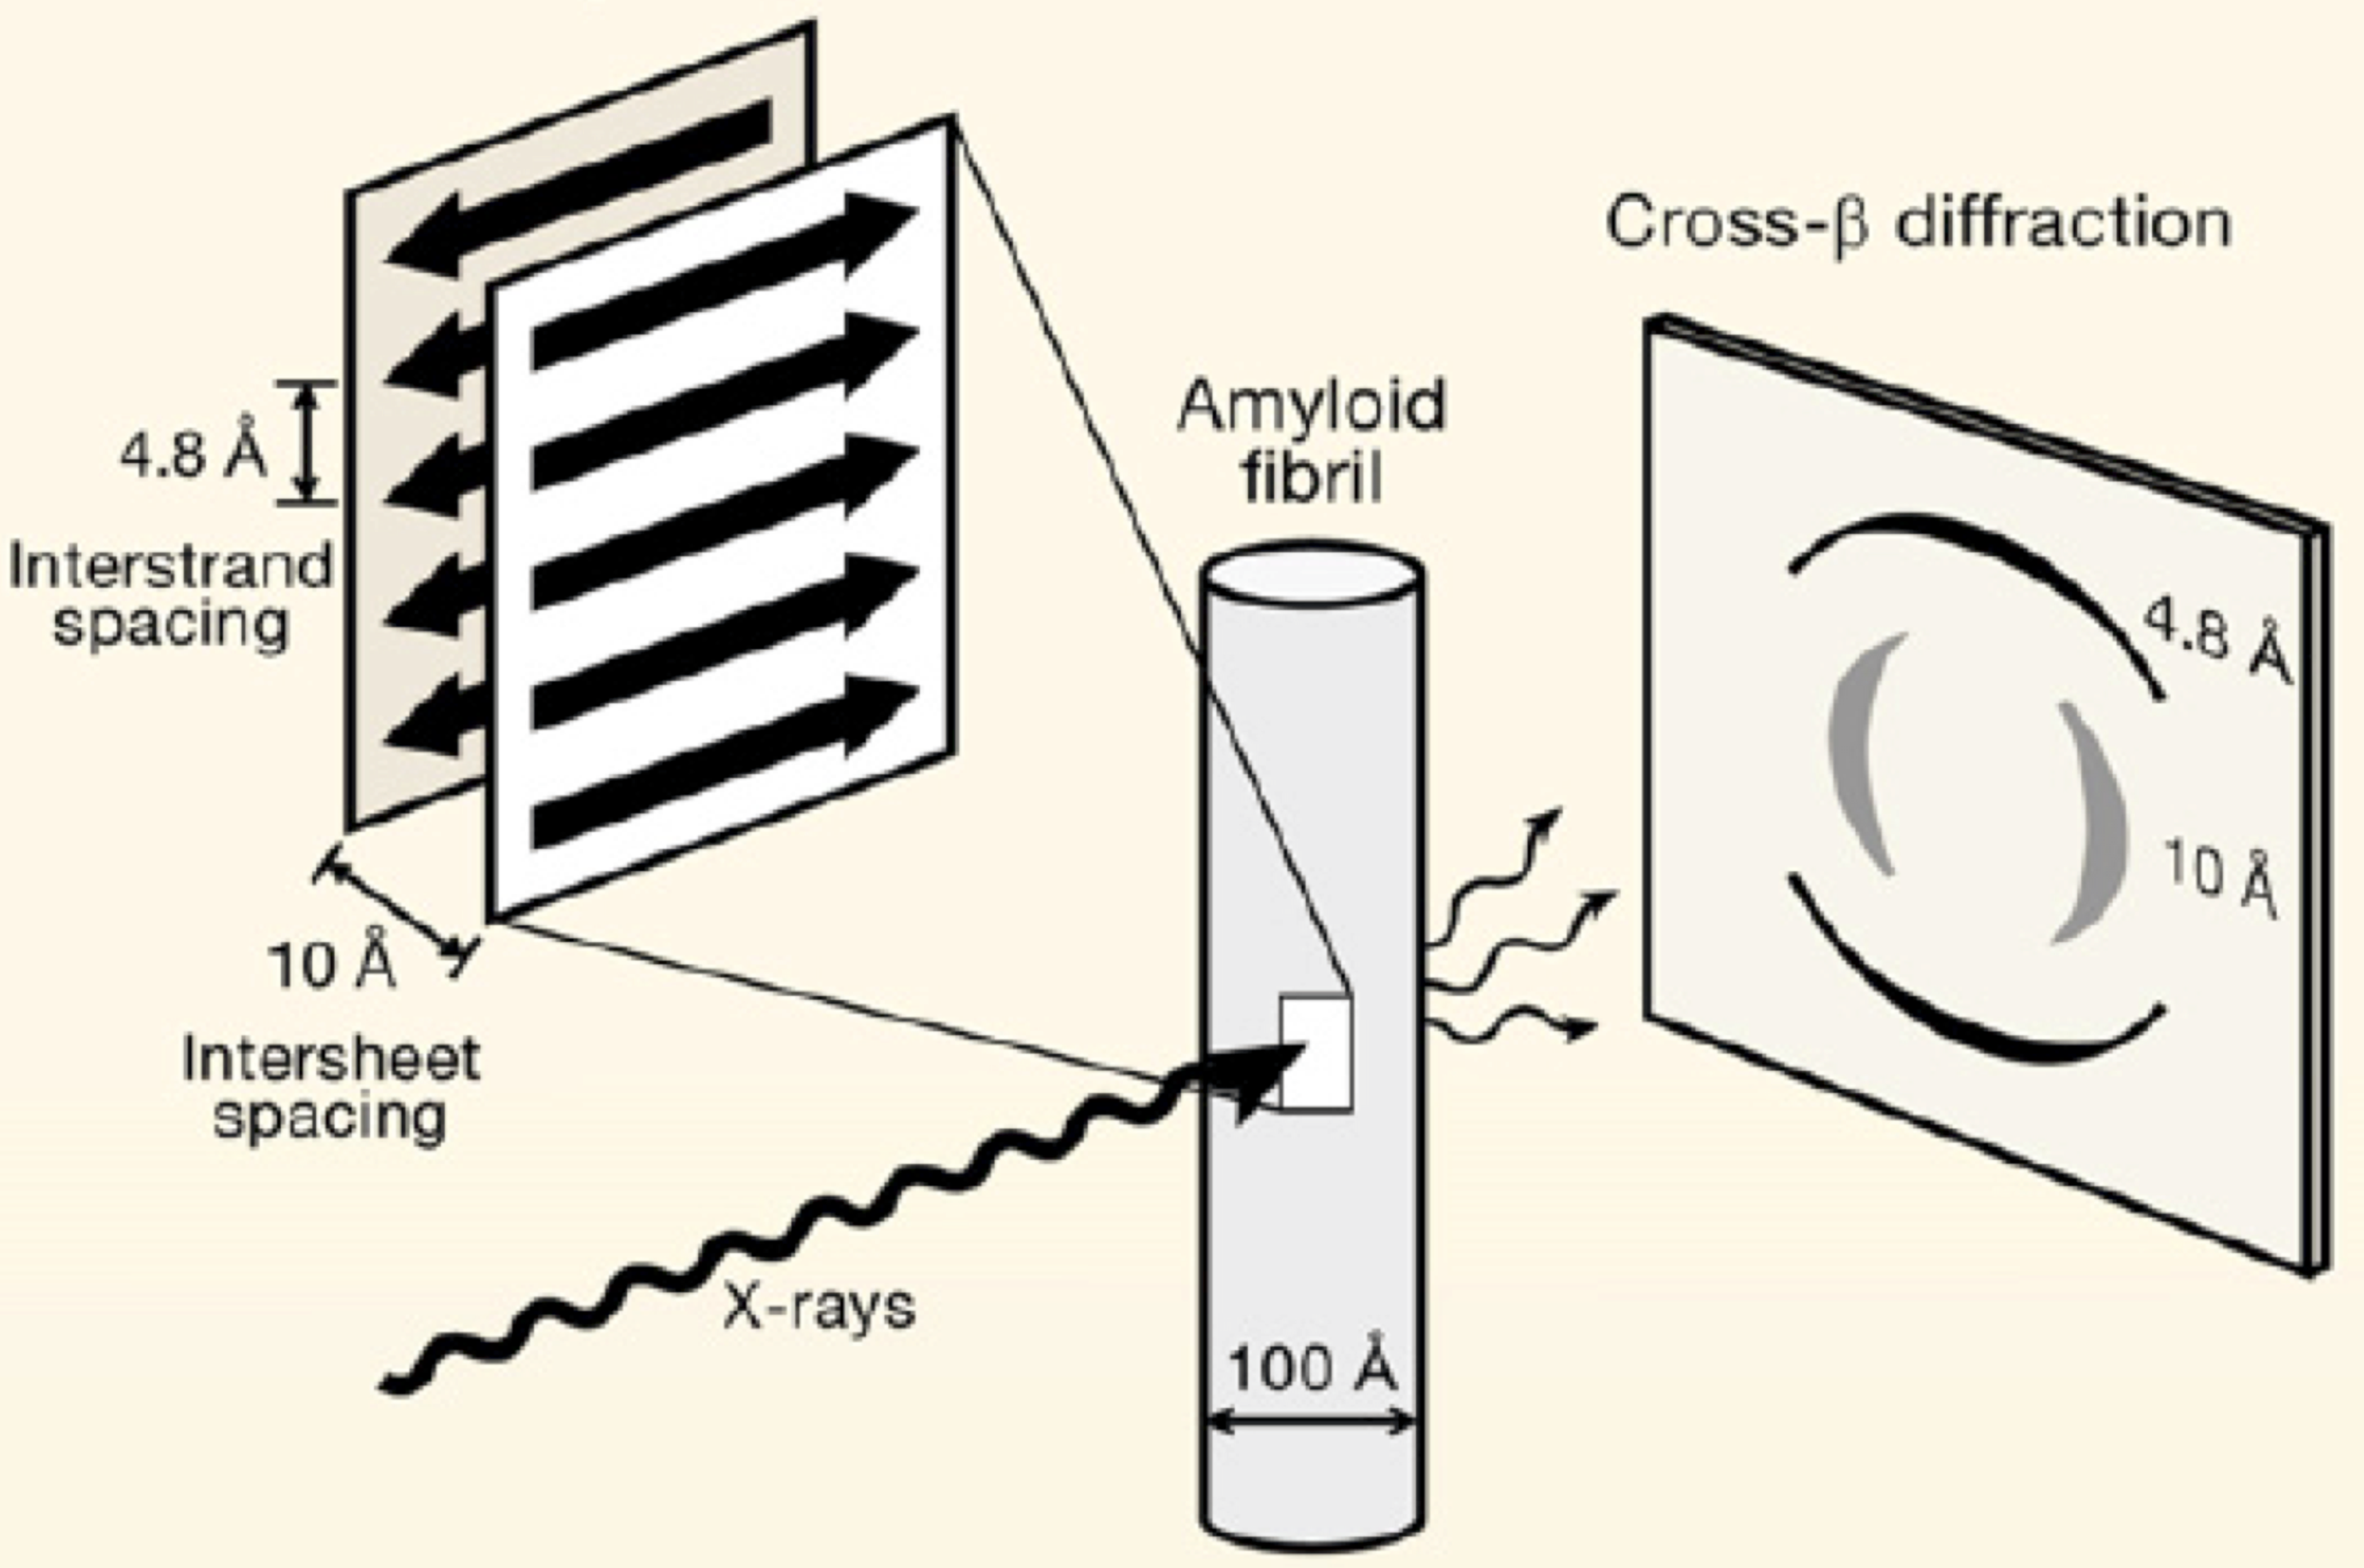
\includegraphics[width=5in]{figures/introduction/fibril_structure_diffraction.pdf}
 \caption[Characteristic cross-$\beta$ spacings from X-ray fibre diffraction studies of amyloid fibrils]{A schematic of the \crossbs\ and the diffraction pattern of fibrils. Reprinted from Cell, 148, D. Eisenberg, M. Jucker, The Amyloid State of Proteins in Human Diseases, 1188 - 1203., Copyright 2012, with permission from Elsevier.}
 \label{fig:fibril_diffraction}
\end{figure}

Amyloid fibrils formed from different polypeptides are thought to share a similar morphology known as the \crossbs.\cite{Chiti:2006fz} To date, independent measurements of fibrillar structure from different instruments have all confirmed the cross-$\beta$ structural core of amyloid fibrils. X-ray fiber diffraction studies showed that the diffraction pattern of fibrils is characterized by major orthogonal reflections along the meridional and equatorial directions, which correspond to a 4.8 \angstrom\ interpeptide separation, and a 10 \angstrom\ intersheet separation, respectively (Figure~\ref{fig:fibril_diffraction}).\cite{Sunde:1997cq,Makin:2005un,Sipe:2000fs} The inter-peptide and inter-sheet separations are respectively parallel and perpendicular to the long-axis of the fibril. This diffraction pattern is now considered as indicative of the presence of \crossbs, and hence, of amyloid fibrils.\cite{Chiti:2006fz} When the fibrils are stained, the macromolecular morphology of fibrils can be determined using the transmission electron microscope (TEM): fibrillar structures are long, unbranched, and ribbon-like structures with diameters between 50 - 100 nm (Figure~\ref{fig:fibril_TEM_SSNMR}).\cite{Chiti:2006fz} 
% Other measurements? - MPL Mass per unit length?

% Although \crossb\ is widely known, due to the insolubility and inherent non-crystalline nature of amyloid fibrils, the molecular details of the fibril structure remained elusive until recent years. 
% The ubiquitous presence of a \crossbs\ supports that the organization of the peptidic backbone, common to all proteins, in to \bsheets\ is a major determinant of the fibrillar structure. 

\begin{figure}
\centering
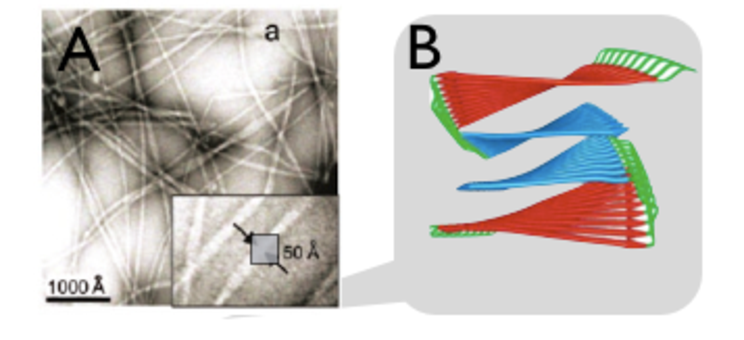
\includegraphics[width=4in]{figures/introduction/fibril_TEM_SSNMR.pdf}
\caption[EM images of amyloid fibrils and oligomers]{(A) TEM image of negatively-stained mature amyloid fibrils.\cite{Petkova:2002p305} Copyright 2002 National Academy of Sciences, USA. (B) SSNMR model proposed by Tycko et al. Reprinted (adapted) with permission from\cite{Petkova:2006gx}. Copyright 2006 American Chemical Society. EM images of oligomers of (C) \abeta42,\cite{Bitan:2003ut} and (D) \abeta40. (C) Copyright 2003 National Academy of Sciences, USA. (D) This research was originally published in Journal of Biological Chemistry. D M Walsh, D M Hartley, Y Kusumoto, Y Fezoui, M M Condron, A Lomakin, G B Benedek, D J Selkoe, and D B Teplow. Amyloid $\beta$-Protein Fibrillogenesis. Journal of Biological Chemistry. 1999; 274:25945-25952. \copyright\ the American Society for Biochemistry and Molecular Biology.}
\label{fig:fibril_TEM_SSNMR}
\end{figure}

\begin{figure}
\centering
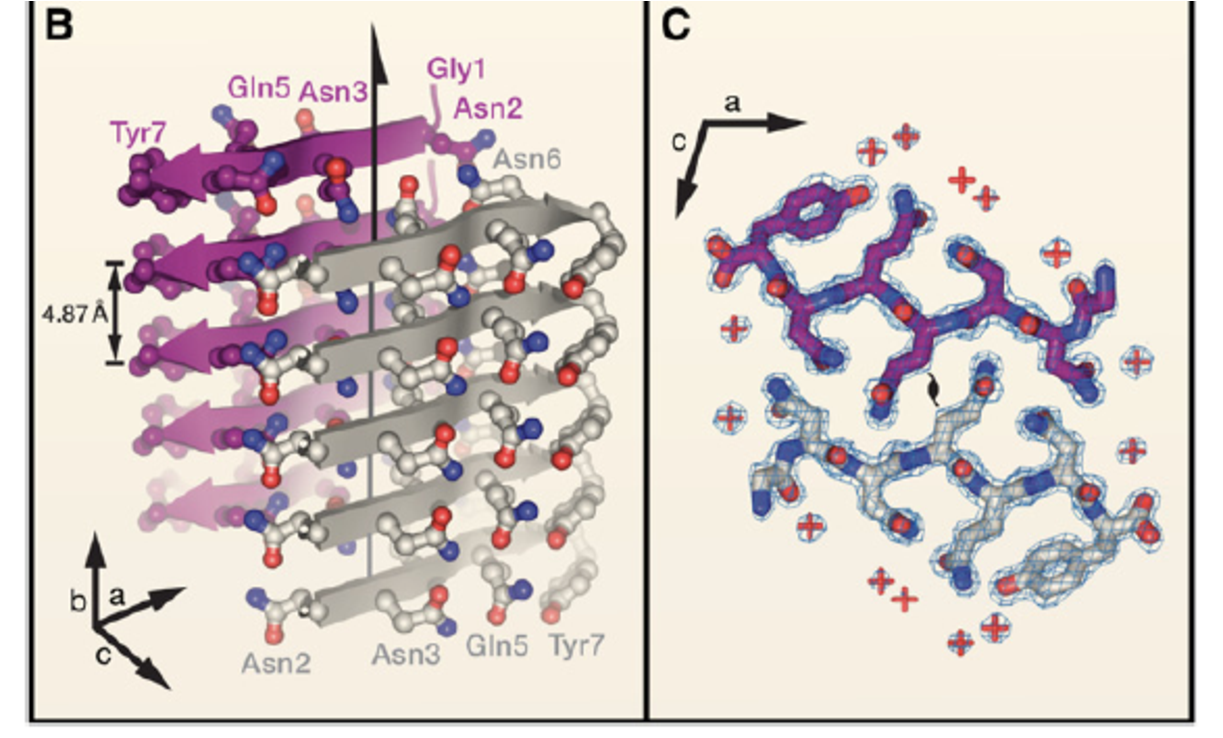
\includegraphics[width=4in]{figures/introduction/fibril_xray_model.pdf}
\caption[X-ray crystal structure of an amyloid fibril]{A schematic of the X-ray crystal structure of fibrils formed from short amyloidogenic peptide fragments. Reprinted from Cell, 148, D. Eisenberg, M. Jucker, The Amyloid State of Proteins in Human Diseases, 1188 - 1203., Copyright 2012, with permission from Elsevier.}
\label{fig:fibril_xray_model}
\end{figure}
% Describe the molecular structure of \abeta\ amyloid fibrils. Briefly mention the techniques that can be used to obtain structural information of amyloid fibrils.
% SSNMR
Advances in solid-state NMR (SSNMR) and X-ray crystallography in the last decade have elucidated the molecular details of amyloid fibrils. One of the first SSNMR models of an amyloid fibril was that of \abeta40, a peptide implicated in Alzheimer's Disease.\cite{Petkova:2006gx}
%The study by Petkova et. al.\cite{Petkova:2006gx} indicated that the \bsheet\ core of \abeta40\ involves residues 10-22 and 30-40, and is linked by a loop formed by residues 23-29. 
Its core fibril unit consists of a parallel in-register \bsheet, where each strand is a \bhairpin\ with peptide-peptide backbone hydrogen bonds running parallel to the long-axis of the fibril (Figure~\ref{fig:fibril_TEM_SSNMR}).\cite{Petkova:2002p305,Petkova:2006gx} In these models, residues 12 to 24 and 30 to 40 of the A$\beta$40 peptide were found to be in the $\beta$-sheet core of the fibril.  Moreover, mutagenesis of residues that disrupts $\beta$-sheet formation in the region of the peptide spanning residues 17 to 23 (Leu-Val-Phe-Phe-Ala-Glu-Asp) can lead to the disruption of the fibrillation of A$\beta$, suggesting that the nonpolar residues Leu-Val-Phe-Phe-Ala constitute the central hydrophobic core of A$\beta$ fibrils.\cite{Wood:1995p2639,Fay:1998vm} Furthermore, smaller fragments of A$\beta$ have been shown to form fibrils that are morphologically similar to those of the full length peptide. For example, A$\beta$(16-22) (or KLVFFAE) have been shown to form amyloid fibrils.\cite{Balbach:2000vf} SSNMR studies of the fibrils of the peptide A$\beta$(16-22) indicated that they are composed of stacked antiparallel $\beta$-sheets.\cite{Balbach:2000vf} Furthermore, fibrils of certain amyloid-forming peptide fragments formed crystals that were amenable to single crystal X-ray diffraction analysis.\cite{Eisenberg:2012hm} In agreement with SSNMR, the crystal structures of these fibrils revealed a structure composed of multiple layers of \bsheet\ with a dehydrated (``dry'') stacking interface (Figure~\ref{fig:fibril_xray_model}).\cite{Sawaya:2007p4363,Eisenberg:2012hm} % Taken together, these recently proposed structures demonstrate that the core region is composed of two to four sheets that interact closely with each other. % I don't think I will talk about the twisting of the sheets too much. Should I mention twisting?
% Fibril polymorphism

The particular packing arrangement of polypeptides in amyloid fibrils can vary with changes in the experimental conditions under which the fibrils are formed. Specific structural polymorphisms include the length of the $\beta$-strands, side chain orientations and inter-protofilament packing.\cite{Kodali:2007cz} Fibril polymorphism may have important implications in amyloid diseases because different morphologies exhibit differing toxicities that depend on which residues are exposed at the surface. For example, \textit{in vitro}, quiescently formed fibrils of A$\beta$(1-40) have been shown to be more toxic than agitated fibrils.\cite{Petkova:2005p4688} 
% A polymorphic structure introduced by a seed have been shown to be able to propagate \textit{in vitro}.\cite{Paravastu:2006p4690} A recent study propagated a brain-derived fibril fragment in order to obtain structural information on fibrils that most closely resembles those formed in the AD brain.\cite{Paravastu:2009fi} -- These points aren't going anywhere.
% http://onlinelibrary.wiley.com/doi/10.1111/j.1742-4658.2010.07888.x/abstract?systemMessage=Wiley+Online+Library+will+be+disrupted+on+15+December+from+10%3A00-12%3A00+GMT+%2805%3A00-07%3A00+EST%29+for+essential+maintenance

\subsection{Non-fibrillar oligomers}

Because of their structural disorder and transient nature, it is difficult to obtain high-resolution structural details of amyloid oligomers using traditional structural determination techniques. Studies using low-resolution techniques transmission electron microscopy (TEM) and atomic force microscopy (AFM) have shown that transient, unstable particles may appear prior to the formation of fibrils (``on-pathway'' oligomers).\cite{Chromy:2003p2575,Ahmed:2010p5694,Caughey:2003jq} These protein aggregates are referred to in literature as amyloid protofibrils.\cite{Chiti:2006fz} Those that do not progress to form fibrils are considered off-pathway.\cite{Kayed:2003en} However, off-pathway oligomers formed in the presence of detergents, lipids, and certain small molecules are typically not considered to be biologically-relevant.\cite{Yu:2009p2873,Laurents:2005ki}
% Oligomers may either be on-pathway to fibril formation, that is, they serve only as intermediates, while others themselves may be the endpoints of aggregation.
% Currently, the precise mechanism involved in the transition from oligomers to extended amyloid fibrils is not known.

Unlike fibrils, amyloid oligomers do not possess a generic structural element and instead, adopt a wide spectrum of sizes and morphologies. Size exclusion chromatography (SEC) studies of \abeta40\ oligomers (isolated \textit{in vitro} and from the brains of deceased individuals with Alzheimer's Disease) revealed the existence of oligomers that ranged in size from dimers to large oligomers of hundreds of peptides.\cite{Haass:2007db,Walsh:2007fu} Oligomeric assemblies that are annular, spherical, or curvilinear in shape have been reported in literature.\cite{Haass:2007db,Kim:2009p2715,Lashuel:2002eg}

% This was directly copied from Fandrich 2012
Although there are large variations in morphologies, oligomers formed from different polypeptide sequences can display similar activities in cell metabolic assays.\cite{Bucciantini:2002un} Importantly, many oligomers of different sizes share the ability to interact with a single oligomer-specific antibody.\cite{Kayed:2003en,Glabe:2008p130} % Large spherical oligomers (3-10nm in diameter) formed from disparate sequences have been shown to binding to a single antibody, which suggests that they may share similar structural elements.
Several studies have indicated that oligomers may possess high $\beta$-sheet content.\cite{Walsh:1999up,Chimon:2007du,Ahmed:2010p5694,Campioni:2010hz} % also bind dyes Thioflavin T (ThT) and Congo Red (CR).\cite{Walsh:2007fu,Haass:2007db,Kodali:2007cz}
Moreover, some non-fibrillar oligomers may contain common structural elements: high-resolution structural studies of non-fibrillar oligomers of \abeta42\ and prion-like peptides suggest that they may contain \crossb\ like fragments.\cite{Walsh:2010p4761,Stroud:2012dp,Chimon:2007du}
 % Should briefly read up on the book chapter by Pat Walsh and cite him
 
% Although oligomers particles may be \bsheet-rich, they are morphologically distinct from fibrils (Figure~\ref{fig:oligomers}).\cite{Walsh:2009p1235}. 
% And may contain random-coil-like conformations\cite{Sandberg:2010ix}

% References for the morphologies from Pat's thesis introd -- (Janson et al. 1999; Conway et al. 2000; Lashuel et al. 2002)
%Conway, K. A., Harper, J. D. and Lansbury, P. T., Jr. (2000). Fibrils formed \textit{in vitro} from alpha-synuclein and two mutant forms linked to Parkinson's disease are typical amyloid. Biochemistry, Vol. 39, No. 10, pp. 2552-63.
%Conway, K. A., Lee, S. J., Rochet, J. C., Ding, T. T., Williamson, R. E. and Lansbury, P. T., Jr. (2000). Acceleration of oligomerization, not fibrillization, is a shared property of both alpha-synuclein mutations linked to early-onset Parkinson's disease: implications for pathogenesis and therapy. Proceedings of the National Academy of Sciences of the United States of America, Vol. 97, No. 2, pp. 571-6.
%Janson, J., Ashley, R. H., Harrison, D., McIntyre, S. and Butler, P. C. (1999). The mechanism of islet amyloid polypeptide toxicity is membrane disruption by intermediate-sized toxic amyloid particles. Diabetes, Vol. 48, No. 3, pp. 491-8.

%\begin{table}%\footnotesize
% \begin{center}
% \vspace{10pt}
% \caption{Summary of proteins which form amyloids}
% \label{tbl:amyloid_diseases}
% \begin{tabular}{| c | c | c | c |}
% \hline
% Peptide & Study & fibrils & oligomers \\
% \hline
% \abeta\ & REFs & yes & yes \\
% alpha-synuclein & REFs & yes & yes \\
% \hline
% \end{tabular}
% \end{center}
%\end{table}

% Outline some of the ideas / hypothesis about the link between amyloid and disease, but don't go into what people speculate or data on toxicity. It is related, but this is out of the scope of your thesis.
% Although not the focus of this thesis, understanding the mechanism of toxicity and elucidating the underlying toxic species will be important in the development of future drug candidates.
%Papers talking about the links of oligomers to disease\cite{Lansbury:2006p928,Lashuel:2006co}
\section{Amyloid involvement in diseases}

Because numerous diseases share the amyloid plaque pathology, fibrils were initially hypothesized to be the toxic species in these diseases.\cite{Hardy:2002dh} However, recent research has implicated non-fibrillar oligomers as the more likely toxic agent in the cause of several neurodegenerative diseases (such as Parkinson's, Alzheimer's, Huntington's diseases and spongiform encephalopathies) and type II diabetes.\cite{Haass:2007db,Xue:2009da,Berthelot:2013fs} % (Baglioni 2006)
Currently, the mechanism of toxicity of amyloid oligomers has not been determined, and is an area under intensive research. Oligomers formed from a variety of peptides, including those not implicated in amyloid disorders (e.g. lysozyme, $\beta$2-microglobulin, transthyretin) all exhibited toxicity, suggesting that the toxicity of amyloid oligomers may be independent of the peptide sequence.\cite{Fandrich:2012kb,Kayed:2003en} Experimental evidence widely supports the hypothesis that amyloid toxicity is based on a generic mechanism that involves the interactions of oligomers with cellular membranes.\cite{Martins:2008bz,Walsh:2007fu} Specifically, it is hypothesized that oligomeric aggregates may ultimately induce cell death by interacting with and disrupting the integrity of the cellular membrane.\cite{Fandrich:2012kb} Moreover, the aggregation of amyloidogenic peptides was found to occur more rapidly in the presence of membrane surfaces,\cite{McLaurin:1997wm,Kayed:2004ul,Yip:2002vx} leading to the claim that membrane-catalyzed fibril formation may induce cellular toxicity.\cite{Yip:2001tl}

% Some studies have suggested that A$beta$ oligomers can increase membrane conductance without the formation of channels.
% Exam question: How does inositol eliminate toxicity of oligomers?

% Table of amyloid diseases 
\begin{table}\footnotesize\centering
    % \begin{center}
    \vspace{10pt}
    \caption{Amyloid-forming peptides and proteins and their associated diseases}
    \label{tbl:amyloid_peptides}
      \begin{tabular}{| c | c |}
        \hline
        Disease & Peptide \\
        \hline
        \hline
	Alzheimer's & A$\beta$40 and A$\beta$42 \\   
        \hline
	Parkinson's & $\alpha$-synuclein \\
        \hline
        Huntington's & poly-glutamine \\
        \hline
        Amyotrophic lateral sclerosis & Superoxide dismutase 1 \\
        \hline
        Spongiform encephalopathies & Prion protein or fragments thereof \\
        \hline
        Type II Diabetes & islet amyloid polypeptide (or Amylin) \\
        \hline
      \end{tabular}
    % \end{center}
  \end{table}


\section{Alzheimer's Disease}
Alzheimer's disease (AD) is a devastating neurodegenerative disease that is the most common cause of dementia in persons of age 65 or older. Upon examination, the post-mortem brains of AD patients show significant neuronal dystrophy. Pathologically, AD is characterized by the presence of extracellular deposits of senile plaques and neurofibrillary tangles (NFTs), both of which appear as lesions on stained neuronal tissue under visible-light microscopy (Figure~\ref{fig:AD_tissue_pathology}).

% Biochemistry of the A$beta$ peptide.
In 1985, the amyloid-$\beta$ protein or \abeta\ was identified as the largest component of these plaques.\cite{Masters:1985wb}
% Review paper on AD from science \cite{Hardy:2002dh}
% C.L.Masters etal.,Proc.Natl.Acad.Sci.U.S.A.82,4245 (1985)
% G.G.Glenner,C.W.Wong,Biochem.Biophys.Res. Commun. 120, 885 (1984).
Monomeric \abeta\ is an approximately 4 kDa peptide produced by the intramembrane proteolytic cleavage of a larger protein, the amyloid-$\beta$ precursor protein (APP).\cite{Hardy:2002dh}
% \abeta\ is produced constitutively as part of the normal cellular metabolism.
APP is sequentially processed by the aspartyl proteases $\beta$-secretase and $\gamma$-secretase, producing a pool of \abeta\ peptides of lengths varying from 38 to 43 residues depending on the position of the cleavage by $\gamma$-secretase (Figure~\ref{fig:AD_abeta_app}).\cite{Gandy:2005dd} The peptides spanning residues 1-40 (\abetaforty) or 1-42 (\abetafortytwo) are predominantly found in AD-associated plaques.\cite{Golde:2000vg,Holtzman:2011gi} Although plaques contain different isoforms of the A$\beta$ peptide, \abetafortytwo\ is likely to be the more deleterious form of \abeta. \textit{In vitro}, \abetafortytwo\ displays significantly higher propensity for aggregation than \abetaforty, despite differing by only two amino acids.\cite{Barrow:1992vz,Jarrett:1993ti,ElAgnaf:2000vr} Furthermore, genetic mutations within presenilin 1 and 2 (genes encoding enzymes that cleave APP to produce A$\beta$ peptides) cause an aggressive early-onset form of AD which also lead to an increase in the ratio of \abetafortytwo\ to \abetaforty\ peptides produced.\cite{Hardy:1997tu,KumarSingh:2006kc,Bentahir:2006ih}

% Pathological characterization
\begin{figure}
 \centering
 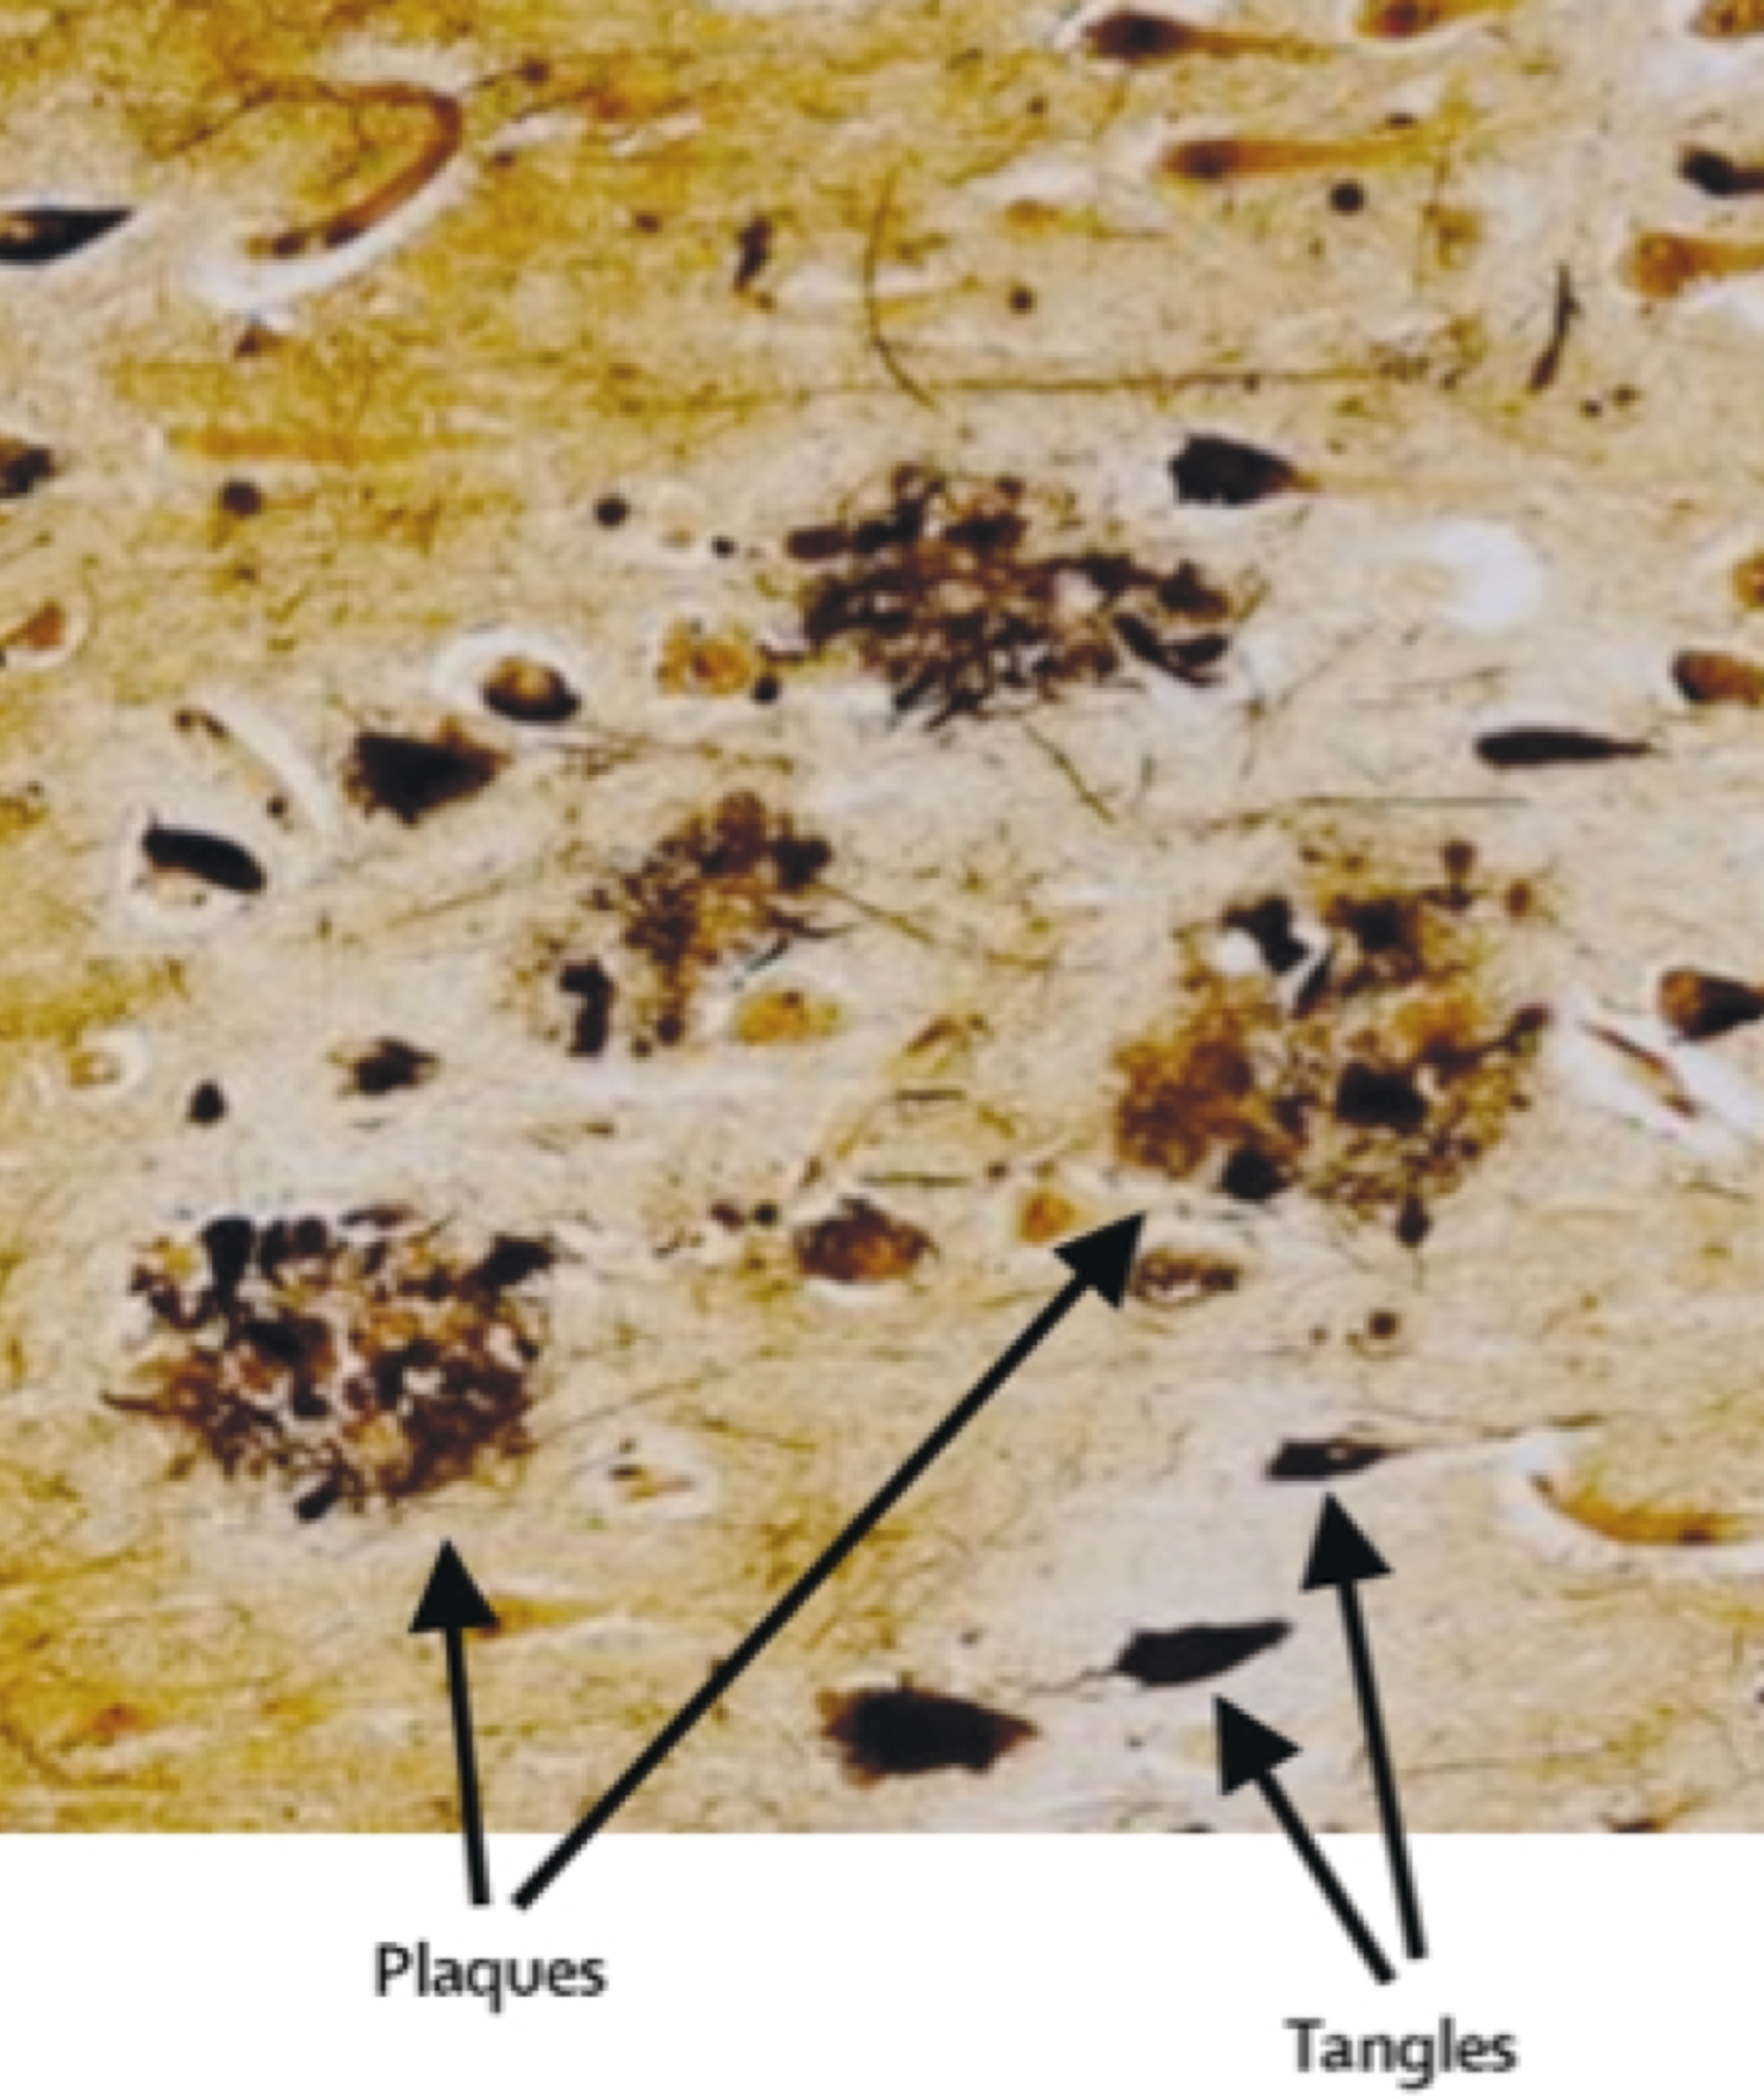
\includegraphics[width=2.5in]{figures/introduction/AD_tissue_pathology.pdf}
 \caption[AD tissue pathology]{Lesions formed from amyloid plaques and NFT tangles in the cerebral cortex tissue of an AD brain. Reprinted from The Lancet, Vol. 368, Kaj Blennow; Mony J de Leon; Henrik Zetterberg, Alzheimer's Disease, 387-403., Copyright 2006, with permission from Elsevier.}
 \label{fig:AD_tissue_pathology}
\end{figure}

\begin{figure}
\centering
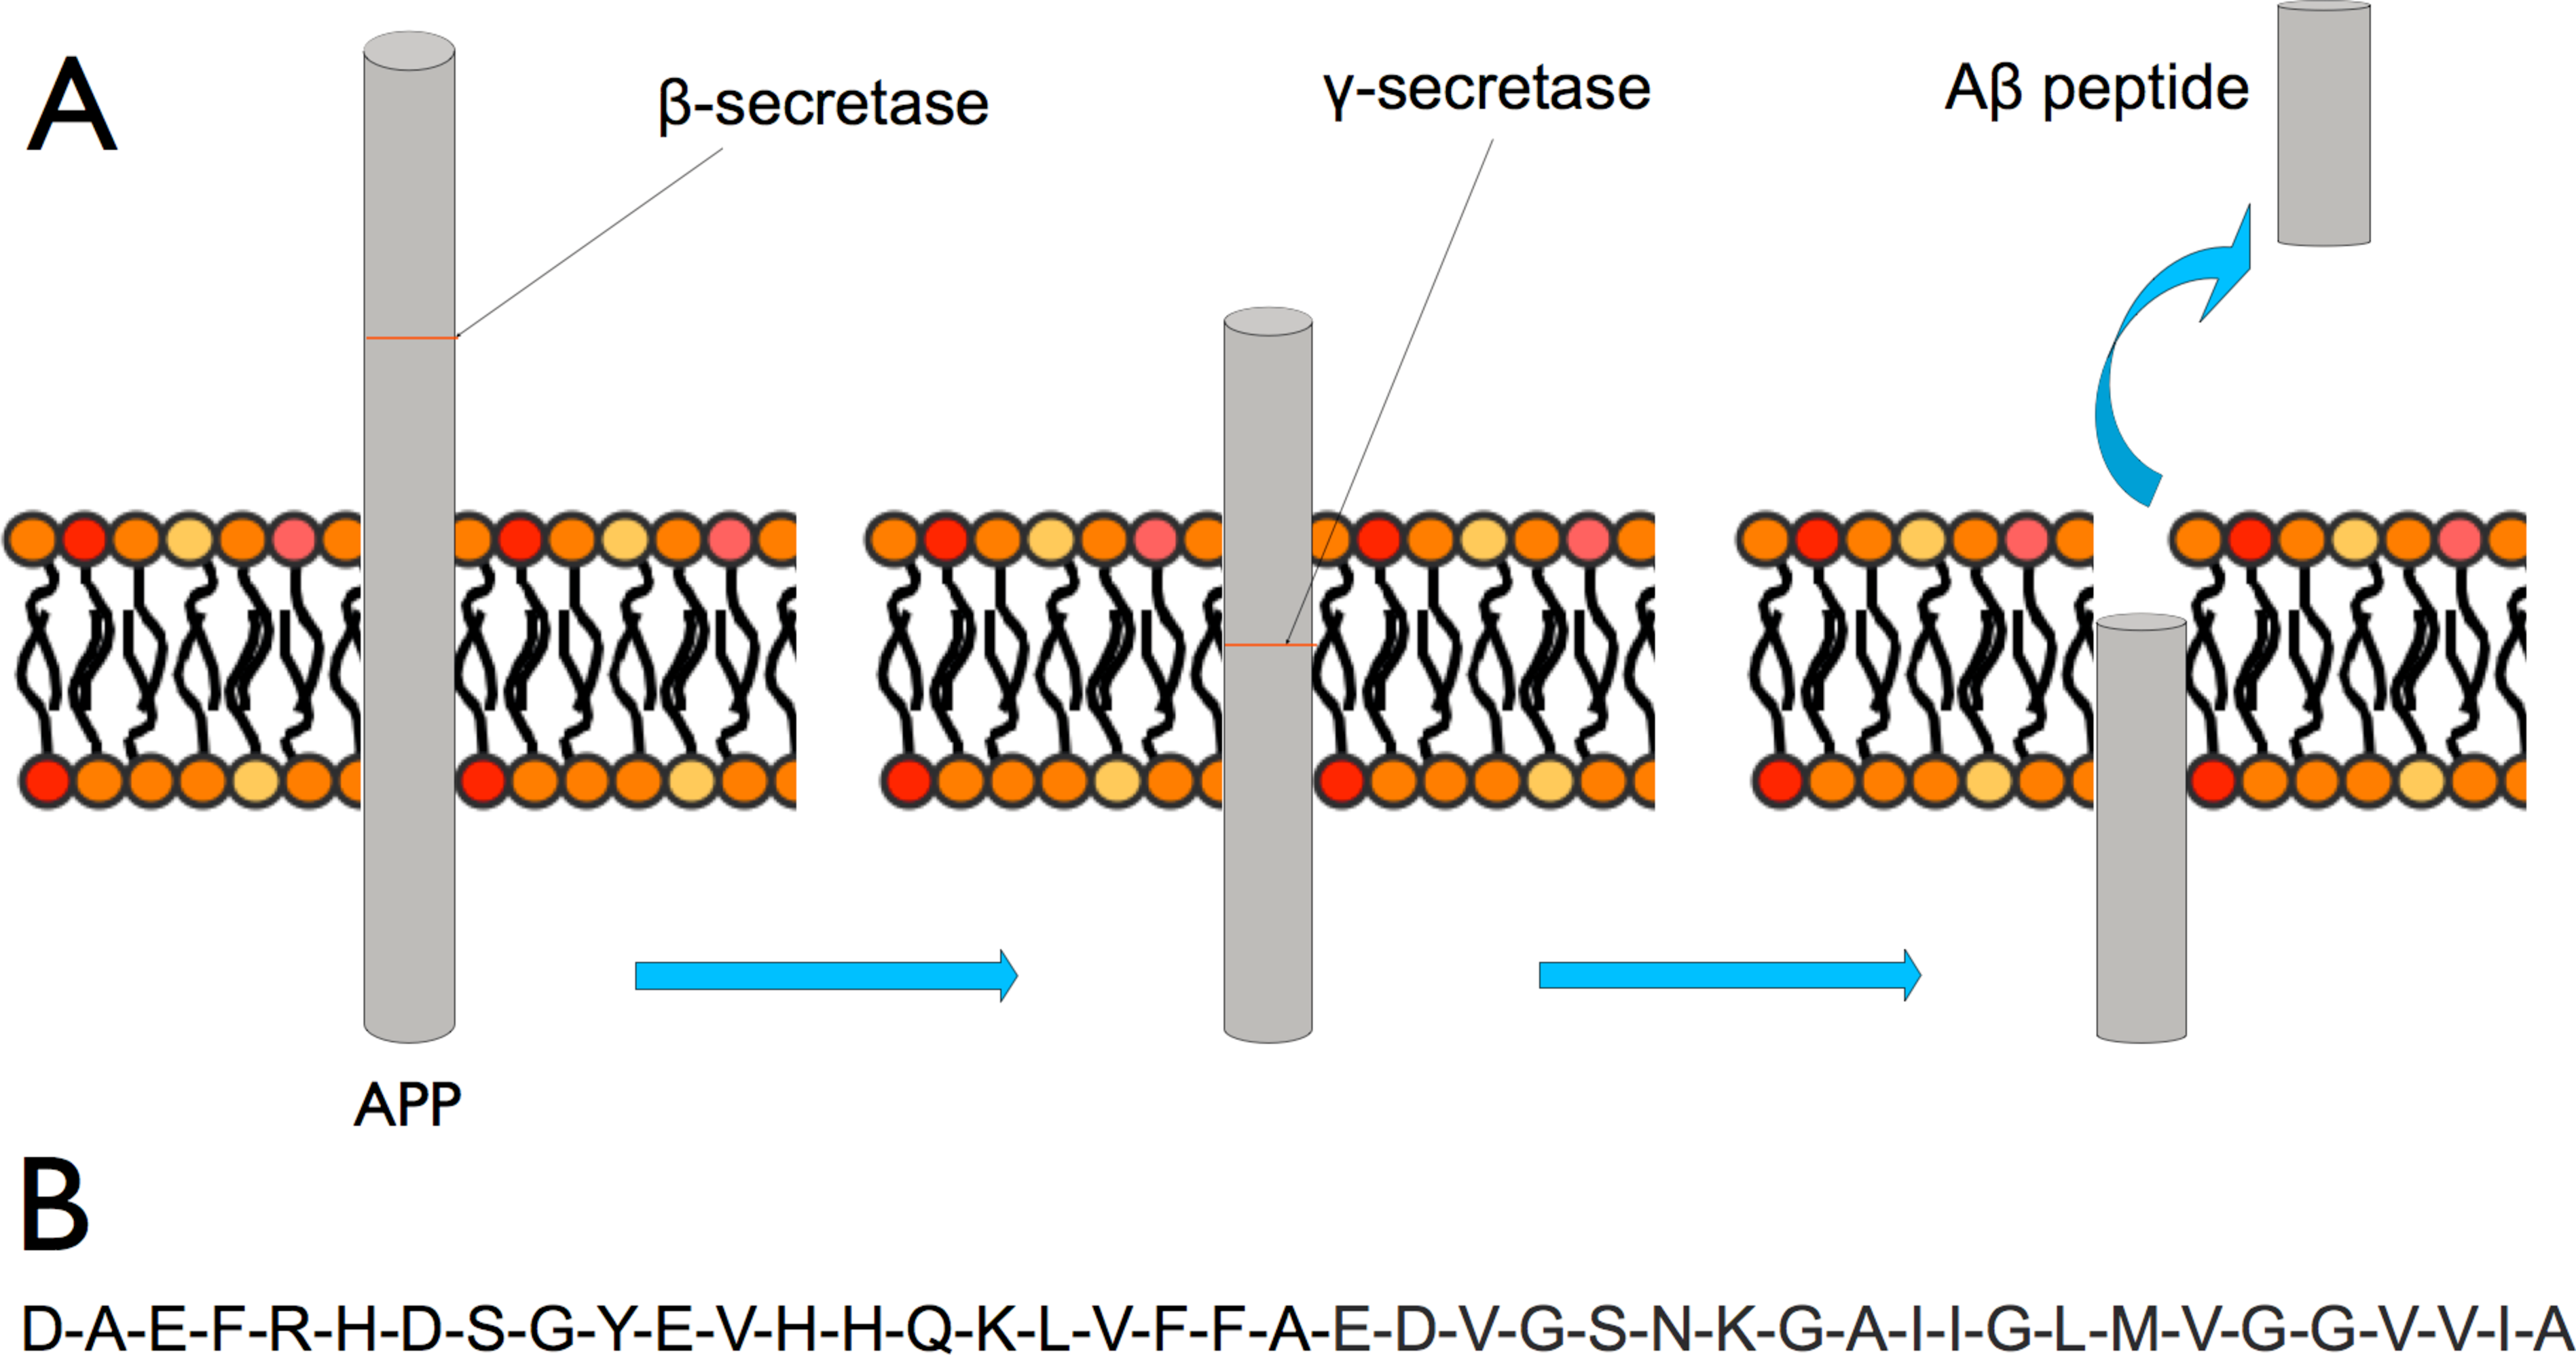
\includegraphics[width=6in]{figures/introduction/AD_abeta_app.pdf}
\caption[APP processing]{A schematic of the production of A$\beta$ via the proteolytic processing of amyloid precursor protein is depicted in (A). The peptide sequence of A$\beta$42 is shown in (B).}
\label{fig:AD_abeta_app}
\end{figure}

% There must be tons of other things that happen in AD .... I’ve made it seem like these oligomers are the only thing that matters.  Perhaps add sentences saying what initiates the disease .. the formation of toxic oligomers. Were the toxicity hypothesis of oligomers for AD have direct evidence from human brain? Look for this. Or was it just pieced together from a bunch of separate animal and cell culture studies? Maybe all of the above.
Although it has been more than one hundred years since Alois Alzheimer first associated the presence of neuronal plaques with the clinical symptoms of Alzheimer's disease, the exact relationship between the two is still under much contention.\cite{Hardy:2002dh} The ubiquitous presence of amyloid plaque deposits found in the brains of deceased dementia patients led to the formulation of the long-standing amyloid cascade hypothesis: the amyloidogenesis of \abeta\ plays a key role in the initiation of AD, which ultimately leads to the clinical symptoms of dementia.\cite{Hardy:2002dh} Genetic evidence provided strong support for the amyloid hypothesis: in those with trisomy 21 (occurring in Down's syndrome), the chromosome responsible for encoding APP, the overproduction of A$\beta$ leads to early-onset of dementia with AD-like plaque load.\cite{Goate:1991kc,LevyLahad:1995vga} Furthermore, in persons with early-onset familial AD, genetic mutations on the APP lead to the production of A$\beta$ peptides with increased aggregation propensities.\cite{Tam:2012vz}
% TODO: Add which mutations -- should I? I have them in a introduction of a chapter.

% Tau protein - Keep discussion brief
In addition to the presence of amyloid plaques, another hallmark of AD is the intracellular deposition of neurofibrillary tangles (NFTs) composed of aggregated hyperphosphorylated forms of the microtubule-associated protein tau.\cite{Ballatore:2007ir} % These tau aggregates have a high $\beta$-sheet content that ultra-structurally appears as paired helical filaments (PHFs) (28, 29).\cite{Holtzman:2011gi}
The role of the tau protein and its interactions with amyloid in the pathogenesis of AD are still being established.\cite{Ittner:2010he} Studies with mouse models currently suggest that the role of NFTs in AD may be downstream to that of \abeta\  because A$\beta$ plaque pathology was not developed in a tau transgenic mouse model, whereas A$\beta$ formation in APP transgenic mice was found to induce hyperphosphorylation of tau, which led to the formation of NFTs.\cite{Gotz:2004dr} 

% A$beta$ and tau review paper -- \cite{Ittner:2010he}
 % More details on evidence which show that NFTs are not likely the causative species.
% I think this detail about abeta aggregation \textit{in vivo} is NICE TO KNOW but could be left out of the thesis.
% The concentration of A$beta$ in the CSF is in the low nanomolar range, but \textit{in vitro} data shows that the critical concentration for aggregation is in the micromolar range. How does it then aggregate in the brain - mechanism of raising the effective concentration.
% \textit{in vitro} models have been useful to screen compound libraries for inhibitors of agregation which may have therapeutic efficacy against AD.

% This was a puzzling aspect of AD which did not fit with the amyloid cascade hypothesis which implicated fibrils as the key cause of toxicity.
A puzzling aspect of AD is that the plaque load in the brain of dementia patients is often not correlated with their disease progression and severity.\cite{Hardy:2002dh,Naslund:2000wf} Instead, multiple lines of evidence indicate that synaptic loss and the severity of cognitive impairment are correlated with the concentration of soluble \abeta\ oligomers in the brain.\cite{Wang:1999fx,McLean:1999ud,Lue:1999vx} For example, oligomers extracted from AD brain can impair synapse structure and function.\cite{Shankar:2008bg}
% Remember to edit this sentence a bit more as I lifted it .. \cite{Tam:2012vz} and references therein.
Moreover, when injected into the brains of animal models of AD, A$\beta$ oligomers decreased the number of synapses and impaired learning performance.\cite{Lesne:2006gx,Cleary:2005kt,Martins:2007bz,Tam:2012vz} Furthermore, cellullar models of toxicity displayed characteristic symptoms of neurotoxicity that lead to eventual apoptosis upon the addition of A$\beta$ oligomers prepared either \textit{in vitro} or extracted from cell cultures.\cite{Cappai:2007bc,Lambert:1998ve,Walsh:2002p2566,Shankar:2008bg,Walsh:2007fu} Taken together, current experimental evidence indicates that preventing the formation of oligomeric forms of A$\beta$ may be a promising method of treatment for AD.
% Don’t go into the structure here ... it was covered before... 
%A variety of morphologically-different oligomers of \abeta\ have been isolated from the human brain, with the smallest of these oligomers dimeric in size (5).\cite{Roychaudhuri:2009iq}
% Are referred to as ``diffuse'' plaques.\cite{Walsh:2007fu} 
% For example, an oligomeric A? species, termed A??56, purified from the brains of mice in an AD mouse model, was found to disrupt memory functions when administered to young rats.
% Lipids have been used to disassemble A? fibrils into smaller structures, which were seen to be highly active in mice.100 
% Key studies which lead to the toxicity mechanisms. Pull some from\cite{Fandrich:2012kb}

% Other review papers for abeta oligomers \cite{Roychaudhuri:2009iq,Sakono:2010kw}
% SDS- stable low-n oligomers of Ab are the fundamental building blocks of insoluble amyloid deposits and could be the earliest mediators of neuronal dysfunction.\cite{Walsh:2007fu}
% Evidence for the involvement of soluble, non-fibrillar Ab in AD has been gleaned through four distinct experimental approaches that utilize (i) synthetic Ab peptides; (ii) cell culture systems in which APP is over-expressed; (iii) APP transgenic mice; and (iv) human CSF and postmortem brain.
% When Ab is deposited and aggregated in a non–b sheet (nonfibrillar) conformation, it is detected via immunohisto- chemical techniques as “diffuse” plaques (Fig. 1C). REF


% Jarrett JT, Berger EP, Lansbury PT Jr. The carboxy terminus of the beta amyloid protein is critical for the seeding of amyloid formation: implications for the pathogenesis of Alzheimer’s disease. Biochemistry 1993; 32: 4693–97. 
% Walsh DM, Selkoe DJ. Deciphering the molecular basis of memory failure in Alzheimer’s disease. Neuron 2004; 44: 181–93.

% In addition, \abetaforty\ and \abetafortytwo\ also have distinct aggregation pathways \textit{in vitro}: \abetafortytwo\ is found to form a morphologically more diverse population of intermediate oligomers than \abetaforty.\cite{Bitan:2003ut} 

% What about mice studies? LOOK AT DAVIS THESIS FOR MORE REFERENCES THERE IN SUPPORT OF ABETA42

% Soluble oligomers - structure? toxicity on cells? rats? mouse?
% What kind of an effect do they have? Synaptic toxicity.

% Take a look at how Lemkul covers this section and transitions to it.
% In this section, I will provide an overview of some of the challenges to overcome when developing a small molecule therapeutic for Alzheimer's disease. Furthermore, using this information, I will motivate why inositol is an exciting avenue to explore.
% Briefly mention non-small molecule putative therapies which also acts via amyloid inhibition. The focus of this thesis will be on small-molecule amyloid inhibition.
% Amyloid inhibition as a treatment for Alzheimer's disease and related amyloid disorders. 
% Talk about how important it is to develop drugs for these amyloid disorders 
\section{Amyloid inhibition by small molecules: a promising method of treatment for AD} 

With the increasing longevity of our population, AD is approaching epidemic proportions and no cure or preventative therapy is available.\cite{Blennow:2006wd} In 2010, it was estimated that 36 million people in the world were suffering from AD, and this number is projected to grow to 115 million people by the year 2050.\cite{alzreport:2012} Furthermore, there are no drugs which may target the underlying disease: approved treatments today such as donepezil (a cholinesterase inhibitor), and memantine (a N-methyl-D-aspartate antagonist) only mitigate cognitive symptoms.\cite{Mangialasche:2010eg}

%\cite{(4) The 2012 PhRMA Report on Medicines in Development: Alzheimer’s disease. See www.phrma.org.} 

% PhRMA reports in their 2012 Medicines in Development Report for AD4 that there are currently 93 medicines in various stages of development, both small molecule and biologic. In general, all 93 compounds fall into one of the following therapeutic strategies: (1) agents targeting neurotransmission, (2) agents targeting Aβ production, (3) agents targeting Aβ aggregation, (4) agents targeting Aβ clearance, (5) agents increasing brain resistance to Aβ, (6) agents targeting tau protein, and (7) agents targeting neurotrophins and agents modulating synaptic plasticity and nerve growth.1−4 \cite{From the ACS neurochem's editorial letter}

% (1) Data from the Alzheimer’s association. See www.alz.org.
% (2) Data from Alzheimer’s foundation. See www.alzfdn.org.
% (3) Mangialasche, F. M., Solomon, A., Winblad, B., Mecocci, P., and Kivipelto, M. (2010) Alzheimer’s disease: clinical trials and drug devleopment’. Lancet Neurol. 9, 702−716. Special Issue: Alzheimer's Disease Published: November 21, 2012
% (4) The 2012 PhRMA Report on Medicines in Development: Alzheimer’s disease. See www.phrma.org. -- I should have a look at this report
% (5) Sadeghi-Nejad, N. (2012) The Lessons of failure: what we can learn from bapineuzumab’s blowup. Forbes (Pharma & Healthcare), August 7, 2012.
% (6) For information of the clinical trials with MK-8931, see www. merck.com.

%\textbf{Need to funnel down to sm inhibition.} 
Although there are currently no therapeutics for AD, progress is being made. Intensive structural and biochemical studies of amyloid structure have led to the development of potential therapeutics for treating the underlying disease. A detailed review of treatment methods which target the underlying disease is provided elsewhere.\cite{Salomone:2012fh} In recent years, small-molecule compounds with the ability to reduce the formation, deposition and accumulation of A$\beta$ amyloid aggregates have emerged as a promising method of treatment. 
%Small molecules which prevent amyloid formation may be an effective method of treatment for amyloid disorders because of the potential to treat the underlying disease. 
\textit{In vitro} screenings led to the discovery of a large number of small molecules that may affect the amyloid aggregation pathway.\cite{Ryan:2012bh} Some of these drug-like molecules inhibit the formation of amyloid fibrils, whereas others arrest or reduce non-fibrillar oligomer formation.\cite{Necula:2007p5049,LeVine:2007jd} % small molecules are thought to act by directly binding to amyloidogenic peptides and aggregates.\cite{Necula:2007p5049} Explain the desirable traits of a drug for AD, and the pharmacological challenges which finding a small-molecule inhibitor of AD presents. 

A key pharmacological requirement of drugs that target AD and other neurodegenerative diseases is their ability to penetrate the blood-brain barrier (BBB) in sufficient concentrations in the brain to achieve their therapeutic effects (i.e., to inhibit amyloid formation).\cite{Hawkes:2009gu,Hubbard:2011fs} Although many small molecules appear to be effective in preventing amyloid formation \textit{in vitro} and attenuating amyloid toxicity in cell cultures, many of these small molecules display poor BBB penetration and are highly toxic, making them unsuitable for immediate use as therapeutics.
% Concentration at which the small molecule acts. BBB penetration and bioavailability.
Below, we provide an overview of small molecules that are \textit{in vitro} and \textit{in vivo} inhibitors of amyloid fibrillation. Clinical trial data is mentioned where available.
% \cite{Necula:2007p5049,LeVine:2007jd}
% review of small molecule inhibition \cite{LeVine:2007jd} \cite{Hard:2012gi}
% Note that here I can take a cue from Justin Lemkul`'s recent review paper.

\begin{figure}
\centering
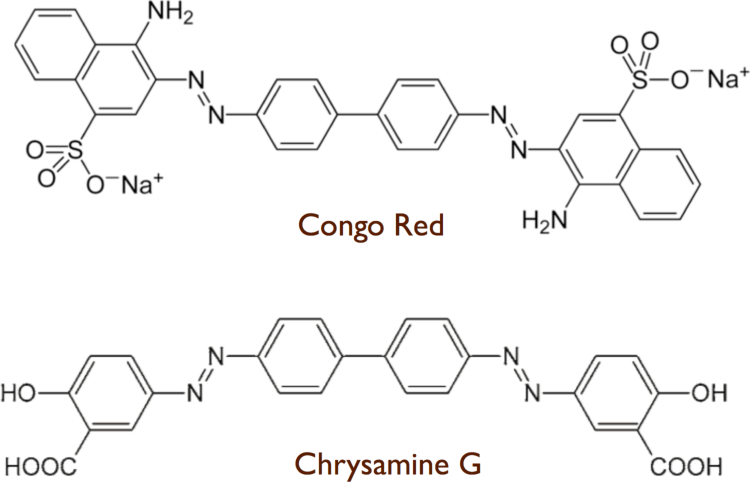
\includegraphics[width=4.5in]{figures/introduction/dyes.pdf}
\caption[Amyloid-binding dyes]{Chemical structure of amyloid-binding dyes Congo red and its derivative, Chrysamine G.}
\label{fig:amyloid_dyes}
\end{figure}

% Questions to answer for the sections below on the various small molecule inhibitors.
% Is it specific to A$beta$ amyloid inhibition? Or fibril structure or what? 
% Any measured concentration of acitivity, IC/EC50, Kd of binding?
% Biophysical data of binding and whether they've been adapted into a drug or were there attempts made to adapt into a drug.
% Molecular mechanism of binding of dye molecules. Thought to bind flat on on the surface grooves of amyloid fibrils where they interact with hydrophobic groups exposed at the surface. 
 % Doesn't explain why the dye molecules are also able to suppress fibril formation.
 % What they are used for ... why one is used over the other. Contrast binding modes, and binding mechanisms, and binding constants. 
 % Make this section tight. Lots of repeat information. Lots of confusing data. Lots of biophysical characterization but still no exact mechanism.
 % Question: Can the birefringence be explained by these binding modes? -- this is out of the scope of my thesis. Don't put this in my thesis but I should be able to coherently explain this during my defense.

% Congo Red (CR) -- DISCUSS ITS PUTATIVE BINDING MODES with amyloid fibrils. What are some binding measurements IC or EC50 values? micro molar? milimolar?

\subsection{Dye-based molecules}

Among the first compounds discovered to bind amyloid fibrils were the dye molecules used to identify amyloids (Figure~\ref{fig:amyloid_dyes}). Congo red (CR) was initially used in the histological detection of amyloid binding, where, upon binding with CR, fibrils exhibit red-green birefringence when viewed with polarized light.\cite{Frid:2007bo} The binding affinity of CR with various fibrils is in the range of 0.1 - 1.5 \micromolar.\cite{Lendel:2009cg,Benditt:1970va,Klunk:1989vc} Like CR, ThT displays \KD's  in the low \micromolar\ range, with values ranging from 0.033 to 23 \micromolar\ reported in the literature.\cite{Groenning:2009p2723} However, unlike CR, although ThT binds tightly to amyloid fibrils, its binding has not been observed to affect amyloid aggregation.  

% The binding affinity of ThT is modulated by physiochemical surface properties of the amyloid fibril: ThT does not appreciably bind fibrils with highly-charged residues such as those of poly-Lysine peptides.\cite{Sabate:2008hb,Khurana:2003dk}

% \textbf{detailed studies}
% \textbf{Putative binding modes of CR molecules with the amyloid fibril are most likely to be bound along the long axis of the fibril. Binding studies where chemical modifications to CR suggest that both ionic and hydrophobic interactions may be important for its binding as disruption of either can affect its binding affinity. Although CR is typically used to detect the presence of fibrillar aggregates, CR may also interact with non-fibrillar conformations such as monomers of alpha-synuclein, and alpha-helical form of poly-L-lysine}.\cite{Maltsev:2012kw} 

Early amyloid detection using CR revealed that CR not only binds to fibrils, but can also affect the amyloid aggregation pathway by interacting with one or more amyloidogenic species.\cite{Caspi:1998vt}
% Add more refs here -- perhaps a general review of congo red binding.
Fibril formation of amyloidogenic A$\beta$ fragments,\cite{Esler:1997bq} prion proteins,\cite{Rudyk:2000ta} and the immunoglobulin light chain variable domain (SMA)\cite{Kim:2003hv} were found to be promoted by the presence of CR at low molar ratios, and inhibited at high molar ratios. 
% \textbf{Not sure if this idea belongs here} Furthermore, it can also self-aggregate in solution to form complexes, which may play a role in its binding mechanism to amyloid peptides and aggregates.\cite{Maltsev:2012kw,Lendel:2009cg}
% Study on CR which shows that it can interact with ThT to interfere with amyloid detection \cite{Buell:2010p9457}

Although CR exhibits anti-amyloidogenic and anti-prion properties, its carcinogenic properties make CR a poor therapeutic candidate.\cite{Hawkes:2009gu} Therefore, efforts were applied to find CR-based analogues that maintain their anti-fibrillar aggregation activity but have improved toxicity profile and BBB bioavailability. Chrysamine G (CG) is one such analogue of CR (Figure~\ref{fig:amyloid_dyes}). CG has higher lipophilicity and lower toxicity than CR, and is capable of inhibiting aggregation and amyloidogenic toxicity both \textit{in vitro} and \textit{in vivo}.\cite{Klunk:1994um,Klunk:1998vm,Reinke:2007p155,Ishii:2002uf}
% lipophilic - ``fat-loving''
% Citations
% A Chemical Analog of Curcumin as an Improved Inhibitor of Amyloid A$beta$ Oligomerization

% Moved ThT binding to the molecular mechanism section.

% Other dye-based inhibitors:
% Methylene Blue is a histological dye molecule (which dye is it based on?) shown to promote the fibrillation of Abeta.
% According to Joanne, it is coming back in clinical trials -- I don't think I need to include this here.
% http://www.ncbi.nlm.nih.gov/pubmed/17595112

% Imaging agents -- I think I should also leave this to good to know. I'm not writing a general review here of the uses of different compounds. I'm talking about what we know about the binding mechanism of various compounds for the inhibition of amyloid formation as a therapy for amyloid disorders.
% In addition to the modification of dyes for the development of therapies, dye molecules have also been used as scaffolds to develop new imaging agents. One such compound is Pittsburgh compound B (PiB), a derivative of ThT, where chemical modifications to ThT led to a much higher binding affinity (in the nanomolar) for amyloid fibrils, and improved BBB penetration.\cite{Raji:2008cv}

% Kill this for now -- Crystallography study of orange-G, a dye-based ...., with amyloidogenic fibril fragments of Tau and Abeta, showed that Orange-G intercalated between sheets by making both nonpolar and electrostatic interactions.\cite{Landau:2011gu}

%\begin{table}%\footnotesize
% \begin{center}
% \vspace{10pt}
% \caption{Summary of small molecules known to affect amyloid formation}
% \label{tbl:inhibitors}
% \begin{tabular}{| c | c | c |}
% \hline
% Molecule & Study & Mechanism of action \\
% \hline
% ThT & REFs & Binding to fibrils \\
% EGCG & REFs & Binding to toxic oligomers \\
%	 \hline
% \end{tabular}
% \end{center}
%\end{table}

% Where are they found? Plants, animals, in food. What are they used for in nature?
% Chemical features of polyphenols? Properties? Soluble?
% What is known about their molecular mechanism?
%\textbf{What other diseases can they treat?}
% for AD
% \textbf{summarize some \textit{in vitro} studies}
% \textbf{summarize some mouse studies}
%\textbf{Their pharmacological properties ... toxicity in the context of treating brain diseases ... }
%\textbf{Has there been any trials using them? Good to indicate here.}
% Curcumin is a flavonoid, resveratrol is not.
\subsection{Polyphenols}
\begin{figure}
\centering
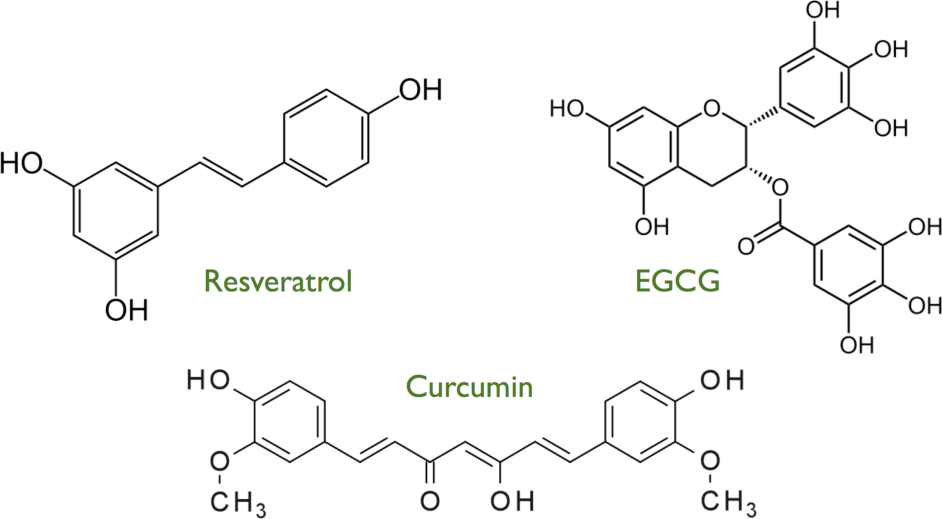
\includegraphics[width=5.5in]{figures/introduction/polyphenols.pdf}
\caption[Polyphenol molecules]{Chemical structures of the polyphenols resveratrol, EGCG, and curcumin.}
\label{fig:polyphenols}
\end{figure}

Polyphenols form a class of molecules found naturally in plants, and are composed of one or more aromatic phenolic rings with multiple hydroxyl groups. Because of their antioxidant properties, the consumption of polyphenols has been reported to be beneficial for health. For example, \resve, a polyphenol found in red wine and \mbox{-epigallocatechin-3-gallate} (EGCG), a major phenolic component of green tea, were found to have cancer-preventative properties.\cite{Baur:2006bx,Singh:2011ec} Currently, several clinical trials which examine their efficacy in cancer treatments are underway.\cite{Baur:2006bx,Singh:2011ec} In recent years, polyphenols have gained additional attention due to their potential for treating AD.\cite{Porat:2006fn} Here we provide an overview of the compounds resveratrol, EGCG, and curcumin, which have been well-characterized for their ability to inhibit amyloid formation.

\textit{In vitro}, \resve\ inhibits the fibril formation of \abeta\ and the islet amyloid polypeptide (involved in type II diabetes), and attenuates amyloid-induced cellular toxicity.\cite{Ono:2008bl,Feng:2009p2240} Similarly, EGCG molecules promote self-assembly of amyloidogenic peptides \abeta\cite{Ehrnhoefer:2008fd} and \alphas\cite{Bieschke:2010ju} into ``off-pathway'' oligomers and inhibit the formation of mature fibrils by directly binding to monomeric forms of these peptides. Cell culture experiments indicate that micromolar concentrations of EGCG are protective against A$\beta$-induced cell death.\cite{Levites:2003wm,Bastianetto:2006du} Curcumin, the main constituent of the spice turmeric, was reported to inhibit A$\beta$ aggregation with IC$_{50}$ values between 0.1-1 \micromolar.\cite{Singh:2012df,Ono:2004td,Hamaguchi:2009p2874,Kim:2005wk} 


% Resveratrol, a polyphenolic molecule found in grapes, red wine and berries, is well-known for its link to the cardioprotective benefits of drinking red wine. 
% EGCG is the major polyphenolic component of green tea, and is well-known for its cancer-preventative effects, which are supported by multiple cell culture, animal, and clinical studies. 
% Resveratrol is current under phase II of clinical trials to determine if resveratrol therapy is beneficial in improving the cognitive function in people with AD.
% Experimental studies of several flavonoids, depicted in Figure~\ref{fig:polyphenols}, are able to modulate amyloid aggregation. Because of their favorable \textit{in vivo} toxicity and high IC50 of inhibition, they have emerged as promising therapeutic candidates for Alzheimer's Disease and related neurodegenerative diseases.


% Studies with AD mice models have suggested that \cur\ can penetrate the BBB in AD.REF
% Although this is the case, \cur\ is likely to have poor bioavailability when administered orally: in rats that were fed \cur\, negligible amounts of the compound were detected in their blood, and high doses were required to attain detectable doses in tissue levels. 

Because of their anti-amyloidogenic activity, low toxicity, and ability to cross the BBB, polyphenols display therapeutic potential for the treatment of AD and related neurodegenerative diseases. Although it is well-known that ECGC, curcumin, and resveratrol inhibit amyloid aggregation \textit{in vitro}, their mechanisms of action are still unknown. A key disadvantage of these polyphenol molecules is their high metabolic activity in the gastrointestinal system, which leads to poor absorption when administered orally.\cite{Baur:2006bx,Smith:2011iq,Hamaguchi:2010wu} Clinical trials to measure their efficacy in the treatment of AD are currently underway.
%Curcumin clinical trials --- Although no adverse events were reported, and the Because these trials only involved a small number of people (between 11 - 34), the effects of \cur\ on cognitive function are inconclusive.\cite{Hamaguchi:2010wu}

% Do they have all similar mechanism of action \textit{in vitro}? 
% \textbf{summarize some \textit{in vitro} studies}
% \textbf{summarize some mouse studies}


%19. Porat Y, Abramowitz A, Gazit E (2006) Inhibition of amyloid fibril formation by polyphenols: Structural similarity and aromatic interactions as a common inhibition mechanism. Chem Biol Drug Des 67(1):27–37.
%20. Ehrnhoefer DE, et al. (2008) EGCG redirects amyloidogenic polypeptides into un- structured, off-pathway oligomers. Nat Struct Mol Biol 15(6):558–566.
%21. Bieschke J, et al. (2010) EGCG remodels mature ?-synuclein and amyloid-? fibrils and reduces cellular toxicity. Proc Natl Acad Sci USA 107(17):7710–7715.
%22. Ladiwala ARA, Dordick JS, Tessier PM (2011) Aromatic small molecules remodel toxic soluble oligomers of amyloid ? through three independent pathways. J Biol Chem 286(5):3209–3218.
%23. Lemkul JA, Bevan DR (2012) Morin inhibits the early stages of amyloid ?-peptide aggregation by altering tertiary and quaternary interactions to produce “off-pathway” structures. Biochemistry 51(30):5990–6009.
%24. Sinha S, et al. (2012) Comparison of three amyloid assembly inhibitors: The sugar \textit{scyllo}-inositol, the polyphenol epigallocatechin gallate, and the molecular tweezer CLR01. ACS Chem Neurosci 3(6):451–458.
%25. Lopez del Amo JM, et al. (2012) Structural properties of EGCG-induced, nontoxic Alzheimer’s disease A? oligomers. J Mol Biol 421(4-5):517–524.
%26. DeToma AS, Choi J-S, Braymer JJ, Lim MH (2011) Myricetin: A naturally occurring regulator of metal-induced amyloid-? aggregation and neurotoxicity. ChemBioChem 12(8):1198–1201.

%\subsection{Non-steroidal Anti-inflammatory compounds (NSAIDs)}
%% Naproxen and ibuprofen
%% From \cite{Takeda:2010gx,Raman:2009jn}
%CUT THIS SECTION DOWN
%
%% I don't think I need to include a whole paragraph summarizing ibuprofen. It's the same story as inositol.
%One of the potential candidates is a nonsteroidal anti-inflammatory drug (NSAID) naproxen and ibuprofen (\ref{fig:nsaids}).\cite{XXX} Epidemi- ological studies have shown that chronic prophylactic intake of naproxen moderately reduces the risk of AD.12,13 Furthermore, reexamination of the results of large-scale clinical trials suggests that under certain conditions naproxen can reduce the AD risk by 67\%.11
%
%Biomedical studies suggest that treatment with ibuprofen reduces the amount of Ab deposits and alleviates memory deficits in mice models (17,18). Ibuprofen intake also correlates with a decrease in the amount of Ab oligomers in mice brain tissues (18). A prophylactic long-term use of ibuprofen appears to reduce the risk of AD (19), but the effectiveness of this drug against preexisting AD cases is unclear (20). 
%
%Several recent experimental studies have investigated the molecular aspects of interactions between Ab and ibuprofen. Binding of ibuprofen to Ab fibrils has been demonstrated when the ligand/peptide stoichiometric ratio approximates or exceeds 1 (21,22). 
%
%Experimental \textit{in vitro} studies have shown that ibuprofen reduces accumulation of Ab fibrils by apparently interfering with fibril elongation (23). Furthermore, ibuprofen demon- strates an ability to at least partially dissociate preformed Ab fibrils (21,23).
%
%\begin{figure}
%\centering
%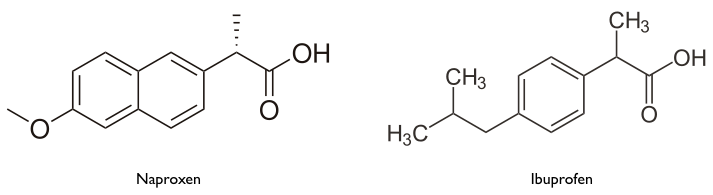
\includegraphics[width=4in]{figures/introduction/nsaids.png}
%\caption[NSAIDs]{NSAIDs}
%\label{fig:nsaids}
%\end{figure}

\subsection{Inositol}
% Here we will review the physiological role of inositol in nature, and introduce inositol as a potential therapeutic for amyloid disorders. Here, use the physiological role of myo-inositol as a lead to transition into its role in amyloid inhibition.
\begin{figure}
\centering
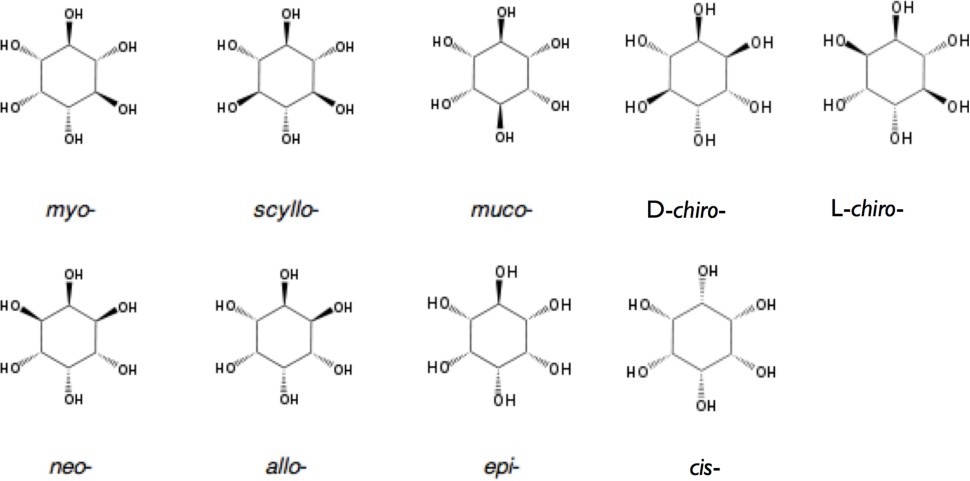
\includegraphics[width=5in]{figures/introduction/inositol.pdf}
\caption[Inositol stereoisomers]{The nine stereoisomers of inositol.}
\label{fig:inositols}
\end{figure}

Inositol or cyclohexane-1,2,3,4,5,6-hexol has the molecular formula \ce{C_6H_{12}O_6}. Inositol is a simple polyol with nine naturally occurring stereoisomers (Figure~\ref{fig:inositols}).\cite{Fisher:2002tk} Out of these nine isomers, seven are optically inactive, and the remaining two (L- and D-\emph{chiro}-inositol) are chiral enantiomers (Figure~\ref{fig:inositols}).\cite{Fisher:2002tk}  The stereoisomers of inositol differ in the arrangement of their hydroxyl groups. In particular, \textit{scyllo}-inositol, with all equatorial hydroxyl groups, is the only isomer that presents two hydrophobic faces. By contrast, its diastereisomer, \textit{chiro}-inositol, with two adjacent axial hydroxyl groups, only has two non-planar faces that are partially hydrophobic. \emph{myo}-Inositol, the most abundant isomer, is ubiquitous in all eukaryotes and is a physiologically important osmolyte.\cite{Fisher:2002tk} Furthermore, \emph{myo}-inositol is a precursor for the synthesis of phosphatidylinositol, an important phospholipid in membranes and second messenger systems.\cite{Fisher:2002tk} Once phosphorylated, \emph{myo}-inositol phosphatides act as second messengers in intracellular signal transduction pathways.\cite{Fisher:2002tk} 
% Add some specific pathways which involves inositol are XXX ... YYY.\cite{Michell:2008dh}

Inositol is found in high concentrations in tissues of the human central nervous system (CNS): \myo\ and \scylloi\ have approximate concentrations of 5 and 0.1 - 0.5 mM in the CNS, respectively.\cite{Fisher:2002tk} Accordingly, inositols also function as osmolytes in the CNS, where alterations in their concentrations are known to be associated with neuropathological conditions.\cite{Michaelis:1993gf,Fisher:2002tk} For example, the pathogenesis of Down's syndrome has been linked to abnormal levels of inositol in the cerebral spinal fluid (CSF).\cite{Fisher:2002tk}

% Role of inositol in amyloid inhibition. Here, include the background on how inositol was discovered as an \abeta\ amyloid fibril inhibitor. Should try to make it into a little story of how inositol was discovered. 
In recent years, \scylloi\ has been identified as a promising therapeutic candidate for the treatment of Alzheimer's disease. Inositol was discovered as a possible amyloid inhibitor in a study where lipid bilayers composed of acidic phospholipids were found to induce $\beta$-sheet structure in monomeric \abeta42.\cite{McLaurin:1996p584} Upon closer examination, \emph{myo}-inositol, the headgroup of phosphatidylinositol, was found to be responsible for the induction of non-fibrillar $\beta$-sheet structure.\cite{McLaurin:1998p3976, McLaurin:1998p3149} This finding led to \textit{in vitro} studies which demonstrated stereochemistry-specific effects of inositol on \abeta\ fibril inhibition and cytotoxicity: \scyllo, \myo, and \epi, but not \chiroi\ inhibit \abeta42 fibril assembly, stabilize an oligomeric complex of \abeta42, and attenuate A$\beta$-oligomer-induced neurotoxicity \textit{in vitro}.\cite{McLaurin:2000bq} Studies with a transgenic mouse model of AD demonstrated that the decrease in their AD-like symptoms after \emph{scyllo}-inositol treatment was correlated with a decrease in the levels of soluble \abeta\ oligomers, suggesting that its beneficial effects are attributed to a reduction in the amount of \abeta\ oligomers.\cite{McLaurin:2006eb}

% I think this is an important paragraph, except I'm not entirely clear on An important therapeutic advantage of \textit{scyllo}-inositol is its ability to readily crosses the blood brain barrier (BBB) (both actively and passively transported). Because it is not enzymatically broken down in the gut, it may be adapted into an orally-administered drug. Although \textit{scyllo}-inositol is found naturally in certain plant organisms and ..., quantities needed for it to be an effective therapeutic is synthesized inside the body ... or can be obtained via nutrition?

Presently, \scylloi\ has completed both phase I and II of human clinical trials for the treatment of AD.\cite{Salloway:2011im} In phase I trials, based on indicators such as brain plasma and CSF concentration, \scylloi\ was found to be non-toxic to healthy individuals at concentrations effective for amyloid inhibition. From 2007 to 2011, phase II studies of \scylloi\ were conducted with three dosage groups, where subjects in each group (comprised of 84 to 91 people) were administered 250 mg, 1000 mg or 2000 mg of \scylloi\ (ELN005) orally twice a day. However, because of greater incidences of serious adverse events at the two higher dosages, only the lower dose was continued. Due to the decrease in the statistical power of the study after the removal of the high dosage groups, the efficacy of \scylloi\ was not conclusively evaluated.\cite{Salloway:2011im} Taken together, these results suggest that \scylloi\ may be a promising therapeutic for the treatment of AD, but that further improvements to enhance its therapeutic properties may be required.\cite{Nitz:2008jl,Sun:2008ko} % Should add something to the effect of ``but further improvements of inositol therapeutics are needed, particularly because they failed clinical trials...''

%\subsection{Commonalities between small molecules}
\section{Protein-ligand binding equilibria}
% Note that I have yet to really find any study with measured Kd or IC50 for amyloid inhibiiton
% These references will help me in part flesh this section out.\cite{Lu:2010jh,Kortagere:2010fc,Nunez:2012il,Copeland:2011dl,Prinz:2008kr,Sikazwe:2012gu,Copeland:2006bb}
Characterizing the binding equilibria between proteins and their ligand substrates is important for understanding the mechanism of action of drug candidates. Binding kinetics describe the rate constants of ligand association (\kon) and dissociation (\koff) for the binding reaction given by
\begin{equation}
% Protein\cdot Ligand \rightleftharpoons^{k_{on}}_{k_{off}} Protein + Ligand
Protein \xrightleftharpoons[\mathit{k_{off}}]{\mathit{k_{on}}} Protein + Ligand
\end{equation}

The ratio of the dissociation to the association rate constants establishes the equilibrium dissociation constant of the ligand ($K_{d}$ = \koff/\kon), which determines the fraction of receptor occupancy at specific ligand concentrations.
 % \2 Absolute binding free energy
 % \2 Relative binding free energy
This equilibrium constant (or the dissociation constant) is

 \begin{equation}
 K_{d} = \frac{\left[ Protein \right]\left[ Ligand \right]}{\left[Protein \cdot Ligand\right]}.
 \end{equation}

$K_d$ is a measurement of the affinity of a ligand for its binding site on the host protein and has units of concentration. Pharmacologically, it is interpreted as the concentration of ligand at which 50\% of the drug is bound to the protein. $K_d$ is often used as a quantitative indication of drug potency when screening for potential lead compounds. $\Delta G$, the binding free energy of a ligand (with its receptor) is directly related to its $K_{d}$ by
 % Free energy equation
%\begin{equation}
%	K_{d} = e^{\frac{-\Delta G}{RT}}
%\end{equation}
\begin{equation}
	\Delta G = -RT\ln K_{d},
\end{equation}
where $R$=1.9858775 x 10$^{-3}$ kcal$\cdot$K$^{-1}\cdot$mol$^{-1}$ is the gas constant, and $T$ is the temperature in the SI unit of Kelvin, and $K_{d}$ is the dissociation constant normalized by the standard molar concentration of 1 mol $\cdot$  L$^{-1}$.

% Binding strength of a ligand to a receptor is often quantitatively assessed by its equilibrium dissociation constants or the Gibbs free energy of binding.
Hence, a small value of $K_{d}$ indicates that the ligand is tightly bound (i.e., it possesses high-affinity binding) to its binding site on the protein, and inversely, a high value indicates weak binding. Enzymes and their inhibitors typically have high binding affinities (or inhibition constants) in the nano- to micromolar range. For example, the nonsteroidal anti-inflammatory drug (NSAID) ibuprofen, which inhibits the enzyme COX-2, displays a \KD\ of $\sim$10 \micromolar.\cite{Cryer:1998ti} 

% Definition and description of binding avidity
In some cases, a ligand may be capable of interacting with its receptor at multiple binding sites. Such ligands may possess weak interactions with several receptor sites, but are able to achieve binding specificity by forming many such weak interactions. An important example of this type of binding mechanism occurs in carbohydrate-protein binding, where multivalency plays an important role in ligand recognition. Binding avidity, distinct from binding affinity,  is a measurement that accounts for all possible binding modes of a ligand with its receptor, and is well-suited for characterizing multivalent interactions such as protein-carbohydrate interactions.\cite{Krishnamurthy:2006vi}

% [Add: the definition of binding avidity constant -- I need to look this up]
\section{Intermolecular forces in biomolecular interactions}

% HBs involved in Binding.
% - What are the energetic contribution of these hydrogen bonds? (How are they measured?)
% osmolytes
% solvent - solvent interactions
% O-H ... O-H

% There lots of different forces; so am I present them as the ones modelled in simulation?
% then I need to mention computer simulation earlier
% Note that I may end up introducing the forces up in the earlier section -- reorganize as needed
% Here, it will benefit me to read Sarah's appendix C carefully.

% Nonpolar
Protein-ligand interactions predominantly involve an array of non-covalent interactions. Van der Waals forces are weak intermolecular forces that are either attractive or repulsive. In particular, London dispersion forces are weak attractive forces between all molecules, which arises from induced correlations of instantaneous dipole moments based on the electronic motions of nearby atoms. In addition, all molecules experience steric effects due to the volume of space that atoms in the molecule occupy. 

Electrostatic effects also play an essential role in biomolecular recognition and structural stability. Fundamental to biomolecular interactions are hydrogen bonding and charge-charge interactions.\cite{Nakamura:1996vm} A hydrogen bond is formed from electrostatic interactions arising between two dipoles: an acceptor and a donor.  The acceptor group is comprised of an electronegative heavy atom (e.g. F, Cl, O), with exposed lone pairs of electrons, and the donor group is comprised of an electropositive atom bound to a hydrogen atom. Furthermore, unlike dispersion forces, hydrogen bonds are directional due to the interaction of a positively-polarized hydrogen and an electronegative atom.  Hydrogen bonds formed between peptide backbones involve N-H and O=C groups as the donor and acceptors, respectively. In liquid and ice water, water molecules form a hydrogen bonding network where a single water molecule may form hydrogen bond with up to four neighboring water molecules (ice).  In this arrangement, the oxygen atom and the two hydrogen atoms of the central water molecule can both form hydrogen bonds with two nearby water molecules.

% [INSERT FIGURE OF GEOMETRY OF HYDROGEN BONDS]
It has been estimated that the dissociation energies of hydrogen bonds range from weak (0.2 kcal/mol) to strong (40 kcal/mol).\cite{Steiner:2002tb} A single water-water hydrogen bond is estimated to have a dissociation energy of approximately 3.2 kcal/mol.\cite{Steiner:2002tb} The energy of a N-H $\cdots$ C=O hydrogen bond is estimated to be -4 kcal/mol in the gas phase,\cite{Klotz:1993fk} and about -0.5 to -1.5 kcal/mol in solution.\cite{Williams:1993wk} %\cite{Sheu:2003jk}
However, the free energy contribution of hydrogen bonding involved in the binding of a ligand and in protein folding is difficult to measure because the energetics of hydrogen bonds are sensitive to the environment in which they are formed.\cite{Klotz:1993fk}
% Note that gas phase measurements are enthalpy only.

% Structure of the DNA ... not only proteins ... should mention this.
Notably, hydrogen bonds are ubiquitous in water, a medium essential to living organisms. A single water molecule is able to tetrahedrally coordinate to four other water molecules to form a network of hydrogen bonds.\cite{Jeffrey:1997ty} This hydrogen-bonded network of water molecules is known to impart to water its uniquely-high heat capacity.\cite{Jeffrey:1997ty} Furthermore, hydrogen bonding plays a key role in stabilizing structures of important biomolecules such as DNA, proteins, and carbohydrates.\cite{Jeffrey:1997ty}In the double-helix structure of DNA,\cite{Watson:1953ug} the complementary base pairing of DNA strands is held together via hydrogen bonding.\cite{Jeffrey:1997ty}

In proteins, intra- and intermolecular hydrogen bonds can be formed between the peptidic backbone, and polar or charged amino acid side chains of polypeptides. Specific hydrogen-bonding patterns define protein secondary structure (such as helices and \bsheets),\cite{Pauling:1951th,Pauling:1950wp} and impart stability to the tertiary structures that are formed by the association of secondary structure elements.\cite{Myers:1996ey} Thus, hydrogen bonding patterns determine the arrangement of peptide strands into either parallel or anti-parallel $\beta$-sheets.\cite{Watson:1953ug} In particular, peptides with their peptidic backbones hydrogen-bonded to each other to form in-register $\beta$-sheets are at the core of the \crossbs\ of amyloid fibrils (see Section \ref{sec:amyloid}).

Salt bridges are considered to be the strongest type of hydrogen bonds in biomolecules. In proteins, salt bridges are a type of hydrogen bond formed between two oppositely-charged amino acid side chains (e.g. arginine and aspartic acid), and are thought to contribute to the overall stability of the protein.\cite{Nakamura:1996vm,Pace:2000eg}

\begin{figure}
 \centering
 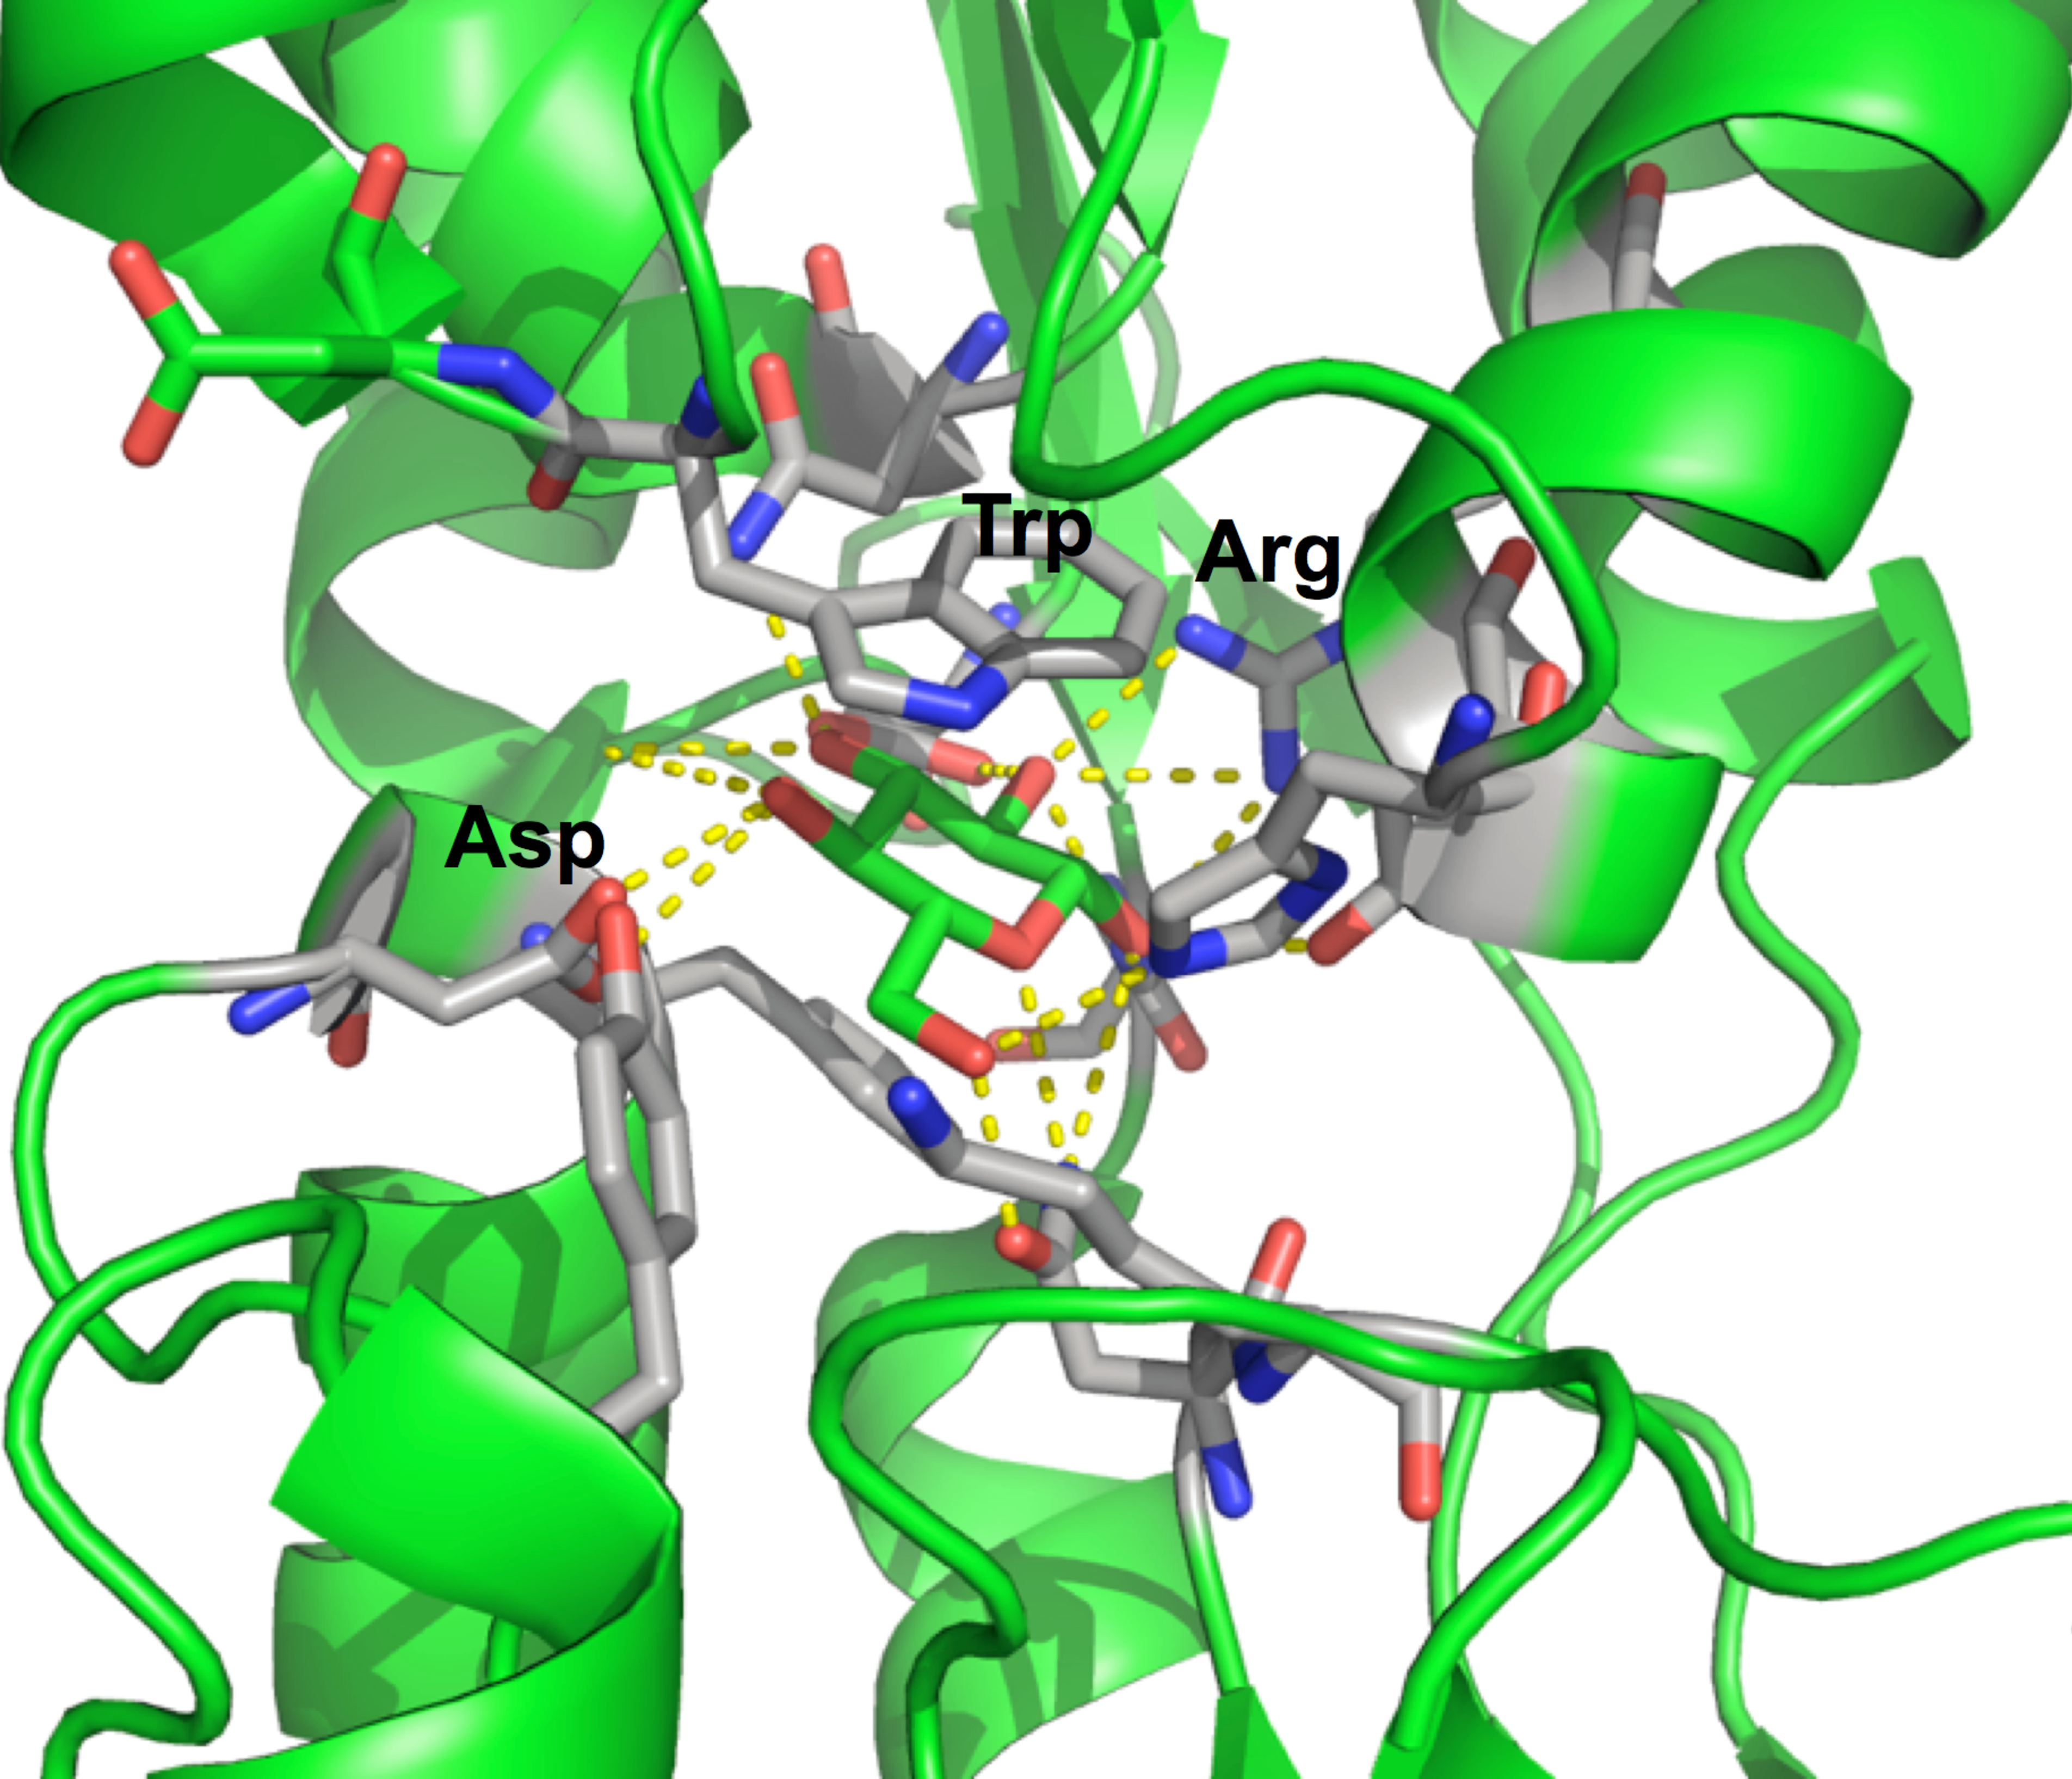
\includegraphics[width=4in]{figures/introduction/sugar_protein_binding.pdf}
 \caption[Example of protein-carbohydrate binding]{Example of protein-carbohydrate binding: glucose bound to a galactose chemoreceptor protein (Ref: Vyas, N. et al, 1991; Rendered from PDB ID: 2GP). Hydrogen bonds between the protein and glucose are depicted in dotted yellow lines. }
 \label{fig:sugar_protein}
\end{figure}

\section{Protein-carbohydrate interactions}
% - Write this section without the cosmic connection
Carbohydrates are the most abundant organic compounds in nature and are an important component of living cells. They are sources of energy, building blocks, and recognition elements for both plants and animals. Proteins capable of binding carbohydrates mediate processes such as antigen recognition by the host immune system,\cite{vanRozendaal:2000fi,Reid:1998tw} signal transduction,\cite{Rudd:2001te} bacterial infections,\cite{Karlsson:1999ta} and cell-cell adhesion.\cite{Rogers:1983wp} 
% Furthermore, carbohydrate-modifying proteins such as glycosyl hydrolases and phosphorylases are of growing importance as potential drug targets. 
Because protein-carbohydrate interactions are involved in many fundamental cellular processes, a great deal of research in the past four decades has been devoted to understanding the molecular basis of their binding mechanism. 
% from \cite{Laederach:2005jh} -- a review of modelling carbo interactions
% Currently, we have a limited understanding of the details of molecular recognition of carbohydrates by proteins, which is critical to a multitude of biological processes. Furthermore, carbohydrate-modifying proteins such as glycosyl hydrolases and phosphorylases are of growing importance as potential drug targets. 

Monosaccharides, or simple sugars, are carbohydrates that cannot be hydrolyzed into simpler sugars. They are building blocks of polysaccharides, which are naturally occurring polymers of monosaccharides. Polysaccharides can be hydrolyzed to form many monosaccharide units.  Smaller polysaccharides of about three to ten units long are sometimes called oligosaccharides. Furthermore, sugars are chiral compounds: a sugar molecule can either be in the D or L configuration. Most naturally occurring sugars are of the D series.

In the past 20 years, the structures of many sugar-binding proteins (or lectins) have been resolved by X-ray crystallography.\cite{Rini:1995p2497} Lectins may have monosaccharides or polysaccharides as substrates. An example of a bound glucose in the active site of its protein receptor is depicted in Figure~\ref{fig:sugar_protein}. Carbohydrate-protein interactions constitute a complex subject. Our discussion here will be focused on the general features of binding sites and binding modes of monosaccharides. 
% Detailed description of various classes of carbohydrate-binding proteins and more complex binding mechanisms are out of the scope this thesis.
% Structural Glycobiology

% Weak binding of carbohydrates
Protein-carbohydrate interactions are relatively weak compared to certain protein-protein interactions. For example, dissociation constants for most lectin-monosaccharide interactions are in the millimolar range, implying that lectins display low binding specificity for their ligands.\cite{Rini:1995p2497} Furthermore, although the affinity increases with oligosaccharides, the dissociation constants are still in the micromolar range.\cite{Zou:1999tn} However, the ability of carbohydrates to form multivalent interactions with their receptors, in part, helps lectins achieve their binding specificity. This mechanism is more generally known as the avidity effect and has been well-documented for several protein-carbohydrate systems.\cite{Rini:1995p2497}

Sugar binding sites are distinct from other ligand binding sites in that they mostly occur at the surface of proteins, and form cavities or grooves. Although any residue may be involved in binding carbohydrates, the most frequently occurring residues are aromatic (Trp, Tyr, and Phe), polar and charged residues (Glu and Asp).\cite{Vyas:1991p6498} Carbohydrate binding sites have been generally classified into two groups: deep, solvent-inaccessible binding pockets and shallow grooves, displaying high and low sugar-binding affinities, respectively.\cite{Vyas:1991p6498,Rini:1995p2497}

\begin{figure}
 \centering
 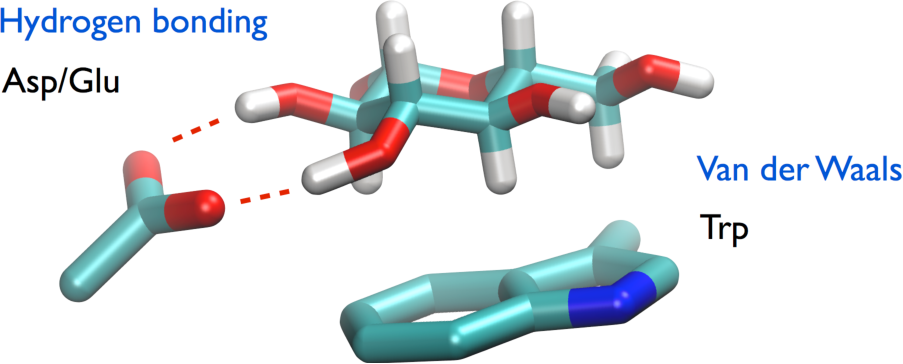
\includegraphics[width=5in]{figures/introduction/sugar_protein_schematic.pdf}
 \caption[A schematic of monosaccharide-protein binding mode]{A schematic of a monosaccharide simultaneously forming Van der Waals interactions with an aromatic moiety (Trp) and bidentate hydrogen bonds with carboxylate group of an acidic residue.}
 \label{fig:sugar_protein_schematic}
\end{figure}

Atomic features of protein-carbohydrate interactions are generally characterized by the concomitant formation of hydrogen bonds and nonpolar interactions with aromatic moieties.\cite{Vyas:1991p6498} Often, a delicate balance between hydrophobic and hydrogen bonding interactions is required for protein-carbohydrate binding, where a slight change in the stereochemistry of the carbohydrate substrate can alter its binding specificity.\cite{Munske:1984ug} % Not sure if this reference is entirely appropriate here.

Because sugars have numerous hydroxyl groups (-OH), hydrogen bonds are ubiquitous in sugar-protein interactions. The hydroxyl groups can interact with both polar and charged groups of amino acids, and the peptidic backbone. A monosaccharide is often found to form planar bidentate hydrogen bonds with the carboxylate groups of aspartic and glutamic acids (Figure~\ref{fig:sugar_protein_schematic}). 
 
Another characteristic binding mode is the nonpolar stacking between hydrophobic faces of the sugar ring and the side chains of aromatic residues (Figure~\ref{fig:sugar_protein_schematic}). This stacking mode, often referred to as CH-$\pi$ interactions, is thought to arise from the entropically favorable packing of the sugar's hydrophobic faces with the protein's aromatic rings, involving enthalpically favorable interactions with $\pi$ orbitals.\cite{Laughrey:2008p6566} % This paper has binding free energies of sugar-aromatic stacking interactions

\section{Structure-based rational drug design}
% The purpose of this paragraph is to connect the pharmacological stuff above? So what? what is next? How do we make new drugs or develop better drugs?  In order to find new drugs it is imperative to understand the mechanism of action of compounds at the molecular level. 
Very broadly, structure-based rational drug design (SBDD) is a process of developing drug candidates by utilizing the structural knowledge of the target protein. With the molecular structure of the target protein, putative enzymatic active sites and other locations that may bind small molecules may be identified.  In SBDD, a target is first identified and its role in the relevant disease pathway is characterized. Then, the molecular structure of the target protein is determined using techniques such as NMR or X-ray crystallography.  If the structure of the target is determined in its ligand-bound state, protein-ligand interactions can be characterized at the molecular-level. Importantly, structural characterization of binding sites facilitates selection and construction of the chemical library for high-throughput screening. Screening of a chemical compound library can be performed to identify ligands (e.g. inhibitors) with high binding affinities (low $K_d$) to the binding site. \textit{In vitro} experiments may be conducted to assess the structure-activity relationship of these compounds. The information obtained from these experiments can either feed back into the design cycle to find better inhibitors, or be used to guide further experiments. SBDD has yielded success in the discovery of drug candidates.\cite{Wlodawer:2002tt,Hubbard:2011fs} Moreover, rational drug design is often applied to optimize ligand binding specificity in an effort to increase the efficacy of the drug candidate, and decrease adverse side effects (toxicity) in the human body.

\section{Molecular dynamics simulations}
% Describe what MD is, then go on to say what one can get from it
% Say at very high level what MD is. Refer to the section for the detailed methods. 
Molecular dynamics is a computer simulation technique which employs an empirical mathematical function to describe the atomic interactions in a molecular system, and, together with classical laws of Newtonian mechanics, predicts the atomic trajectory of motion of a molecular system. Thermodynamic and kinetic properties can then be extracted as time averages from these trajectories and used to make a number of predictions that are often experimentally challenging to observe or measure. 

In general, MD simulations are a useful tool to study the structure, dynamics, and interaction of biomolecules (see Chapter 2 for methodological details). MD simulation studies have been useful in studying many existing fundamental problems of biology and biochemistry, including protein folding, biomolecular self-aggregation, and protein-ligand binding.\cite{Karplus:2002wt} With increasingly faster and cheaper computer hardware, and better algorithms, structure-based computer modelling and simulations of protein-ligand interactions are becoming a key component of the modern drug discovery process. For example, MD simulations can predict protein-ligand binding free energies, a quantity that can be used to evaluate how well a ligand binds.\cite{Rodinger:2005dw,Rodinger:2008p5581,Gilson:2007hz}

Alternative \textit{in silico} methods such as computational docking, where the energetics of binding is typically estimated without accounting for either ligand or protein flexibility, can provide a crude estimate of ligand binding affinity.\cite{Abagyan:2001un,Wei:2004fu} Although docking is fast, its inaccuracy often leads to many false positives. In MD simulations, the protein and its putative ligand are allowed to relax and freely move about in the system, allowing a more realistic estimate of the binding free energy. Simulation trajectories of protein-ligand binding can be used to quantitatively assess whether a chemical change to a compound will produce a more potent drug candidate (e.g. residues may be ``mutated'' in silico).\cite{Kim:2006hy,Schwab:2008ia}

\subsection{Challenges and limitations of MD simulations}
% For that to happen we either have to sample the necessary timescales or find a way to bypass the energetic barriers which separates 

For molecular simulations to reliably predict and guide experiments, they need to be sufficiently accurate, include a correct representation of the experimental conditions, and adequately sample the relevant biomolecular motions.\cite{Mobley:2011ks} Ideally, a simulation should be at least 10 times longer than the slowest important timescale in a system.\cite{Zuckerman:2011dz} However, it is often difficult to sample events on the timescales relevant to many important biologically-relevant phenomena (e.g. protein folding, amyloid formation, ligand binding and conformational isomerization) because their timescales (typically greater than 1 ms) are often not attainable via brute-force MD simulations using currently-available computing resources. Although modern simulations studies routinely approach microseconds in sampling, only a few studies to date were able to reach timescales of milliseconds.\cite{Dror:2012cs,Shan:2011bo,LindorffLarsen:2011gl}

Consequently, running a single continuous MD simulation alone is unlikely to achieve sufficient sampling of the important states of many biologically relevant systems. For this reason, computational algorithms which enhance sampling of the energy landscape of biomolecular systems are often employed to overcome some of the limitations of conventional MD simulations.\cite{Rauscher:2009wr}

% However, in the case of understanding a specific binding reaction often needed when developing an enzyme inhibitor, the ability to observe the relevant binding events is a low probability event on the timescale achievable by simulations. Therefore, a few enhanced techniques have been developed to accelerate this process. They are briefly introduced below.

% MD simulations can also be used to rapidly prototype experimental ideas -- for example, one can perform computational alchemy, that is, ``mutate'' residues to test various hypotheses. 

\section{Recent progress in elucidating the molecular mechanism of small-molecule binders and inhibitors of amyloidogenic species}
% How is small molecule binding different from the classical ligand-enzyme binding paradigm? 
% Why is finding small-molecule inhibitors for amyloid is different from finding enzymatic inhibitors. 
% [Are most drugs identified in that way?] Although the structure-based rational drug discovery paradigm is well-suited to finding inhibitors of globular proteins such as enzymes, designing small-molecules which may inhibit amyloid formation presents additional challenges. -- I think this statement leads the reader to believe that SBDD is the only way to find drugs.

Amyloid fibrillation is a multi-stage process involving different species at each stage. Due to the heterogeneous nature of prefibrillar species, experimental determination of the molecular structures of these amyloid species remains a challenge. Further compounding experimental challenges, these small molecules may interact with amyloidogenic species at different stages of aggregation, which are not known \textit{a priori}. Moreover, the binding mechanism of small-molecule inhibitors of amyloid aggregation is not described completely by the classical enzyme-inhibition model.  An inhibitor concentration in the micromolar to millimolar range is often required to observe amyloid inhibition,\cite{Hawkes:2009gu} suggesting that these \smis\ are non-specific binders. By contrast, substrates of folded enzymes exhibit higher binding specificity, with binding affinities frequently in the nanomolar range.\cite{Liu:2007dk} Taken together, the above challenges have significantly impeded the determination of the molecular basis of amyloid inhibition by \smis\ using existing experimental methods. 

By contrast, computer simulations are not limited by these experimental challenges and can provide the atomistic level of detail needed to elucidate the action of small-molecules on the inhibition of amyloid formation.
% Don't make it seem like its just easily done using MD. Challenges of small molecule simulations ....
As a result, MD simulations have played a key role in advancing the understanding of the binding mechanism of these small-molecule inhibitors. However, elucidating the molecular basis of these \smis\ poses a number of difficulties for simulation studies. The structural disorder of amyloid-forming peptides makes it difficult to obtain statistically-meaningful properties from MD simulations. Furthermore, because it is not known whether \smis\ may interact with amyloidogenic monomers or aggregates, it is often necessary to examining their binding with several amyloidogenic species in order to gain a complete understanding of their mechanism of action.

% \textbf{Lemkul: Targeting A? aggregation presents a considerable challenge. That is, how can the ability of a compound to bind A? be assessed when the target peptide undergoes large and continual conformational changes? This type of information is difficult to gather using traditional experimental techniques and thus represents an area well suited to theoretical methods (21). Information obtained from molecular dynamics (MD) simulations will likely accelerate the process of novel Alzheimer’s drug development and has recently been successfully employed in designing A? aggregation inhibitors (22). Here, we summarize and evaluate current progress in application of docking and MD studies and give perspective on the future of these techniques in the development of compounds that may inhibit A? aggregation and thus serve as potential therapeutic agents against Alzheimer’s disease.}
% Although many \smi\ were found to have activity in affecting amyloid formation, only a limited number of them had their binding mechanism examined by MD simulations. 

% CN commented this out because you don't do this.. at least not "below".... Perhaps GL wants to add this back but clarify where the reader will find this information.
% A large number of MD simulation studies were published between the years of 2007 to 2013 (the time of research reported in this thesis). 

% Notes: 
% What exactly should I cover in my reviews?
% Explicit solvent? Is this too much detail?
% Extensive simulations? Simulation times?
% Conventional MD? Special tricks were used?
% Force field?
% Concentration / molar ratio
% statistics?

A large number of MD simulation studies were published at the time of research reported in this thesis. Below I will provide a review of the recent progress in elucidating the binding mechanism of small molecule inhibitors of amyloid formation. While the central focus of the review is on MD simulation studies, experimental results are discussed if they are available.
Both \textit{in silico} methods and experimentally-tractable model self-assembly systems have provided significant insight into the binding modes of small molecules with amyloid fibrillar aggregates. MD simulation studies examined the binding of Congo red (CR) with the protofibril of the amyloidogenic fragment GNNQQNY of the yeast prion Sup35,\cite{Wu:2007p361} and most recently, with full-length \abeta40.\cite{Shea:2012eh} Although protofibrils of \abeta40\ were found to contain more binding sites for CR than GNNQQNY, CR shared similar binding modes with protofibrils of both peptides: CR molecules bound in the fibrillar grooves, between peptide strands, in parallel to and perpendicular to the long-axis of the fibril, respectively.  These results led the authors to hypothesize that the observed $\beta$-sheet surface binding mode disrupts $\beta$-sheet stacking, whereas edge binding (found exclusively with \abeta40\ fibrils) blocks strand-to-sheet extension.  Moreover, based on these binding modes, a model for explaining the birefringence displayed by A$\beta$ fibrils upon binding CR was proposed.\cite{Shea:2012eh}

To identify the minimal requirements for ThT binding, Biancalana \textit{et. al.} designed a set of novel ThT-binding proteins to create a minimalist binding site for ThT that recapitulated all of its fibril binding properties (i.e. fluorescence emission upon binding).\cite{Biancalana:2009p5056} The X-ray crystal structure of the $\beta$-sheet protein containing high-affinity binding sites for ThT showed that its surface contained repetitive grooves formed by tyrosine (Tyr) and leucine (Leu) arranged in a side-by-side manner (``ladders'').\cite{Biancalana:2010p5053} Based on this structure, the authors hypothesized that ThT preferentially binds to aromatic grooves at fibrillar surfaces. Wu  \textit{et. al.} later conducted a complementary MD simulation study of this model ThT-binding protein which corroborated this hypothesis.\cite{Wu:2009p1954}
% and a crystal structure of a model ThT-binding protein.\cite{Wu:2009p1954}

In several MD simulation studies, Wu \textit{et. al.} examined the binding of ThT and its analogs to protofibrils of A$\beta$(16-22)\cite{Wu:2008ds} and full-length A$\beta$40 peptides.\cite{Wu:2011fd}   These studies revealed that similar to the binding modes of CR, ThT was bound to several binding sites located on the surface of fibrils.  Furthermore, the results of their studies suggest that although CR and ThT share similar binding site motifs, they are not likely to share similar binding sites because of differences in their chemical structure and variations in the surface properties of fibrils.

Taken together, the above studies suggest a consensus for the molecular mechanism of dye binding to amyloid fibrils: dye molecules adopt specific binding modes in the grooves at the surface of amyloid fibrils, which give rise to the physical properties exhibited by dye-bound fibrils. However, it is still not understood why CR binding leads to amyloid inhibition, but ThT binding does not. Further investigation of the differences in their binding mechanisms will be required.
% Although their binding predominantly depends on the amyloid fibrillar structure, it can depend on factors such as physicochemical surface property of fibrils.

Using a combination of isothermal titration calorimetry (ITC), NMR, and MD simulations, the interaction of \mbox{-epigallocatechin-3-gallate} (EGCG) molecules with monomeric \abeta42\ as modulated by temperature, pH, salt concentration, and ligand:protein molar ratio was investigated by Wang \textit{et. al.}\cite{Wang:2010p5887} The simulations were performed in the presence of EGCG, at increasing molar ratios, with the A$\beta$ peptide in $\alpha$-helical conformation.  Results of this study indicated that both hydrogen bonding and hydrophobic (aromatic) interactions are important for binding of EGCG, and that the balance of these interactions is particularly sensitive to ligand:protein stoichiometry.

The molecular details of EGCG binding to A$\beta$ monomers were further explored using MD simulations, exclusively, in a follow-up study\cite{Liu:2011ka} using a similar simulation protocol as in the previous study.\cite{Wang:2010p5887} Using MM-PBSA,\cite{Kollman:2000vm} a technique that employs continuum solvent models to estimate binding free energies, the authors found that nonpolar interactions rather than hydrogen bonding contributed more to EGCG binding modes.
% (\textbf{did they provide a number ... was this based on energetic analysis?}).
Furthermore, based on secondary structure analysis of the peptide conformations, EGCG, at ligand:peptide molar ratio of 10:1, was found to prevent $\beta$-strand formation.

Binding modes of morin, a polyphenol molecule with the ability to inhibit amyloid formation of A$\beta$ and IAPP peptides \textit{in vitro},\cite{Hamaguchi:2009p2874}\cite{Noor:2012fc} were investigated with protofibrils of \abeta42\ using MD simulations by Lemkul \textit{et. al.}\cite{Lemkul:2010bf} Based on contact analysis and snapshots from simulations, morin predominantly bound at the edges of the protofibril, and partially penetrated the hydrophobic interior of the protofibril.  Furthermore, in a significant fraction of the simulations, morin molecules hydrogen-bonded to and intercalated between a pair of residues which formed salt bridges within the fibril.

% TODO: These simulations were non-equilibrium - no convergence
% TODO: Check that the inter and intra peptide contacts are what they consider to be tertiary and quaternary contacts
% TODO: Re-read this paper ...
In a follow-up MD study, the same authors investigated the effect of morin binding on the aggregation and conformational equilibria of monomers and dimers of \abeta42.\cite{Lemkul:2012jn} Morin was found to bind to the residues flanking the central hydrophobic core region (CHC) of the A$\beta$ peptide (residues 16 to 21), but not with the CHC itself.  Morin-peptide interactions were found to  impede the formation of intra- and inter-peptide hydrophobic contacts, but did not affect the secondary structure of the peptide.   On the basis of these results, the authors proposed that morin prevents fibril formation of \abeta42\ by preventing and disrupting the hydrophobic association to form an initial aggregation nuclei.

NSAIDs, typically administered for pain relief, are also found to inhibit A$\beta$ fibrils \textit{in vitro}.\cite{Agdeppa:2003us,Hirohata:2005kc}  In a series of MD simulation studies, Klimov \textit{et. al.} examined the binding mechanism of ibuprofen\cite{Raman:2009jn} and naproxen\cite{Kim:2011fn} with monomers, oligomers and protofibrils of \abeta40. In each of these studies, replica-exchange MD simulations, an enhanced sampling simulation methodology, were conducted to increase the likelihood of NSAID-A$\beta$ binding events. To reduce time required for their simulations, an implicit solvent model was used in place of representing water molecules explicitly.

The authors found that ibuprofen preferentially binds to the protofibril rather than to the monomer of \abeta40, predominantly in the hydrophobic grooves at the edges of the protofibrils.\cite{Raman:2009jn}  This protofibrillar binding mode of NSAIDs was speculated to inhibit fibril formation by blocking fibril elongation.\cite{Raman:2009jn} Furthermore, a comparative study of naproxen and ibuprofen was carried out to identify the molecular basis of naproxen's stronger \textit{in vitro} binding affinity.\cite{Takeda:2010gx} Although both NSAID molecules share binding sites on the fibril, naproxen was found to have higher binding energy than ibuprofen because of its preference for self-interaction.\cite{Takeda:2010gx}
% TODO: https://www.pivotaltracker.com/story/show/63666842
% TODO: Missing link. Need to re-read this paper.  Will leave out for now because I just want to get the draft over to RP. The authors proposed that naproxen may interfere with A$\beta$ oligomer formation by intercalating between associating monomeric peptides.\cite{Kim:2011fn} 

% Based on the results of that study, simulations of dimers of Abeta40 were conducted with naproxen to further examine its binding modes with disordered forms of amyloid aggregates.\cite{Kim:2011fn} 

% Discuss after Klimov's study descriptions. Discuss other possible issues with implicit solvation models. Some studies use implicit solvation only.  Note I know nothing about this and I don�t think I�ll have enough time today to write this up. -- Need citations.
% \textbf{In summary}, there is an emerging picture of small molecule binding from simulation studies when pieced together with the \textit{in vitro} data.
% [Should these be concluding paragraphs or opening? I feel like they read as concluding because now that you�ve gone through the studies.  But from another angle, it would make reading the detailed reviews easier for readers because now they are guided rather than getting lost in the details of the studies. Furthermore, it is easier to justify not providing an exhaustive review. This is quite similar to how David structured his review section in his thesis. But then I don't think it makes sense to discuss hypothesis without having introduced what was studied in the first place]

In summary, the above simulation studies suggest that both hydrophobic and hydrogen bonding interactions are involved in the binding mechanism of known \textit{in vitro} small molecule inhibitors. Based on MD simulations, several mechanistic hypotheses for the molecular mechanism of amyloid inhibition by small molecules have been put forth.  First, it has been hypothesized that  fibril formation may be prevented by binding to surfaces of $\beta$-sheet aggregates.\cite{Jiang:2011hf,Shea:2012eh}  Furthermore, many small-molecule inhibitors are thought to interact with multiple species along the amyloid formation pathway.  For this reason,  simulation studies were conducted to examine the interaction of small molecule inhibitors with peptides and protein monomers and non-fibrillar amyloid aggregates.\cite{Kim:2011fn,Lemkul:2012jn,Liu:2011ka} These studies suggest that small molecules prevent peptide self-aggregation by interacting with amyloidogenic aggregates and displacing their $\beta$-sheet-forming propensity.\cite{Kim:2011fn,Lemkul:2012jn,Liu:2011ka} % there were a whole bunch others, but I wasn't able to review them.

Despite the continued increase in computational power, modern MD simulations of disordered proteins and peptides remain computationally challenging.\cite{Rauscher:2010p5682}  For this reason, the conclusions drawn from these simulations may suffer from systematic or statistical sampling errors that are difficult to identify. Thus far, studies of small molecule binding lack statistically significant numbers of binding events, due to the lack of sufficient sampling time. Hence, dissociation constants (\KD), which are an important metric of a compound's efficacy in the rational drug design process, have not been estimated from simulation studies.  Without an estimate for the \KD,  the relevance of the binding sites identified in simulation studies are more difficult to assess because direct comparisons with \emph{in vitro} measurements cannot be made.

% Move this down to a later discussion - In each of these studies, a large amount of sampling on the order of tens of microseconds were devoted to understanding of NSAID binding.
An implicit solvation model may be used in place of explicit solvent representation in order to reduce computational complexity of the simulations.\cite{Feig:2004jd} Some of the studies referred to above have employed this methodology to examine small-molecule binding mechanisms.\cite{Kim:2011fn,Takeda:2010gx,Raman:2009jn} However, the lack of explicit solvent, an important contributor to the free energy of ligand binding,  can lead to quantitative errors in binding mode predictions. Certain models of implicit solvation introduce approximations to account for these effects, but are much less accurate in reproducing them.  % Nevertheless, the authros derived interesting results which may help further our understanding of small molecule binding...

Few studies conducted currently are systematic comparative studies of monomers, disordered oligomers, and protofibrillar aggregates. Because it is often not known which amyloidogenic species these small molecules may act on, the lack of adequate comparisons may leave a study susceptible to biased mechanistic hypotheses. Moreover, experimental studies have suggested that the activity of these small molecules is modulated by their concentration and molar ratio. For example, the self-aggregation of small-molecule binders at high concentrations has been reported in both experimental\cite{Feng:2008fj,Maltsev:2012kw,Lendel:2010p3376} and simulation studies.\cite{Liu:2011ka,Takeda:2010gx,Raman:2009jn} However,  the mechanistic link of this effect to their mechanism of amyloid inhibition has not been addressed by most studies.

% Many studies do not address reversible binding.
Amyloidogenic monomers and oligomers can adopt a large number of comformational states, and requires a large amount of computational sampling in order converge their conformational properties in order to determine the effect of small-molecule binding on their conformational equilibria. Hence, to reduce simulation time, several MD studies have utilized smaller fragments of the A$\beta$ peptide.\cite{Convertino:2011epa,Convertino:2009ce,Chebaro:2012ba} 
% Furthermore, recent studies have begun to perform MD simulations in combination with enhanced sampling methods to probe binding of small molecules with full-length peptide monomer of A$\beta$.  
However, many existing studies in the literature, particularly those which probe the effect of ligand binding on conformation of monomers and oligomers of the full-length A$\beta$ peptides, draw conclusions based on non-equilibrium simulations where the conformational property of interest likely remains unconverged.\cite{Liu:2011ka,Convertino:2009ce,Lemkul:2012jn}  Due to the lack of assessment of convergence in these simulations, researchers have been unable to assess the statistical significance of their data, which could lead to significant systematic biases. 
% I think I�ll skip this point for now to because I don�t really review too many of these
% (I think there was a study by Derremaux that recently used RE and measured convergence. -- I�m not sure if I�ll include this point.)
% Punchline: Then *bam* say my study is complete �  Segue into Thesis objectives.

\section{Thesis objectives and organization}

% These paragraphs are taken from HPCS and sound sexier than the one that I had from before.
One out of eight people aged 65 or older has Alzheimer's disease (AD).\cite{Citron:2010p4427} With the increasing longevity of our population, AD is approaching epidemic proportions with no cure or preventative therapy available.  A pathological hallmark of AD is the extracellular deposition of amyloid in the brain.  These fibrillar deposits (plaques) are formed from the self-aggregation of the $\beta$-amyloid (A$\beta$) peptide, a 38 to 42 residue protein that is produced normally as part of the cellular metabolism.  Similarly, amyloid composed of other peptides or proteins are also found in other neurodegenerative diseases such as Parkinson's, Huntington's, and prion-related diseases.

One therapeutic approach is the development of small-molecule inhibitors of A$\beta$ aggregation. Recently, \textit{scyllo}-inositol has emerged as a promising compound for the treatment of AD, which has currently completed phase two of clinical trials. It is one of eight stereoisomers of inositol found in nature and exhibits stereochemistry-dependent inhibition of A$\beta$ fibrillation.\cite{McLaurin:2000bq} \textit{Scyllo}-inositol is effective at reversing the established disease state as well as preventing the onset of AD-like symptoms in a transgenic mouse model of AD, whereas \textit{chiro}-inositol is inactive.\cite{McLaurin:2006eb}  Currently, \textit{scyllo}-inositol has completed phase two of clinical trials, which evaluates its dose-related safety and efficacy in participants with mild to moderate AD.

% \textit{Scyllo}-inositol is a promising potential therapeutic compound for AD treatment,  \textit{Scyllo}-inositol has been shown to effectively block the accumulation of A$\beta$ oligomeric assemblies and reduce AD-like symptoms in a transgenic mouse model of AD. Furthermore, \textit{in vitro}, \textit{scyllo}-inositol and its stereoisomers \textit{myo}-inositol, \textit{epi}-inositol and \textit{chiro}-inositol, have been demonstrated to stabilize A$\beta$42 oligomers, disassemble preformed A$\beta$42 fibrils, and reduce A$\beta$42-induced neurotoxicity in a stereochemistry-dependent manner. \textit{Chiro}-inositol is a stereoisomer that was shown to be inactive in inhibiting amyloid formation. 
Although \textit{scyllo}-inositol raises hope for the development of a cure for AD, it is likely that effective therapies for patients with AD will require rational modification of this compound. Understanding the molecular basis for the action of inositol and in particular, its effect on A$\beta$ aggregation will aid in the effective development of inhibitors of amyloid aggregation. At present, however, experimental approaches lack the ability to determine the precise mechanistic modes of action of inositol as the molecular structures of various intermediates in the A$\beta$ aggregation pathway are not known. Moreover, intermediate states in the fibriillation process are very difficult to detect and isolate by experimental methods.
% However, the specific molecular interactions of inositol and its effect on A$\beta$ aggregation at the molecular level are not known.

The primary objective of my research is to use MD simulations to elucidate the molecular basis for the activity of inositol by determining its effect on the structure and thermodynamics of A$\beta$ aggregation. Our central hypothesis is that inositol acts by binding to one or more of the aggregated form of A$\beta$. The formation of amyloid follows a complex aggregation pathway, where different intermediate A$\beta$ aggregate species have been implicated in the disease. Small molecule inhibitors such as inositol may interact with species at various stages of aggregation. Therefore, a meaningful study requires examining inositol binding with different self-aggregated peptide states, from monomeric to fibrillar aggregates. To this end, I have carried out systematic comparative studies of amyloidogenic peptides and their aggregates of increasing sequence and composition complexity and characterized the respective role of specific interactions of inositol with the backbone and sidechains (Figure~\ref{fig:rationale}). In all of my studies, I have comparatively examined \textit{chiro}- and \textit{scyllo}-inositol with each of the aggregates in the pathway to determine the stereochemical basis of the activity of inositol. In addition, I also performed control simulations in the absence of inositol.  

\begin{figure}
\centering
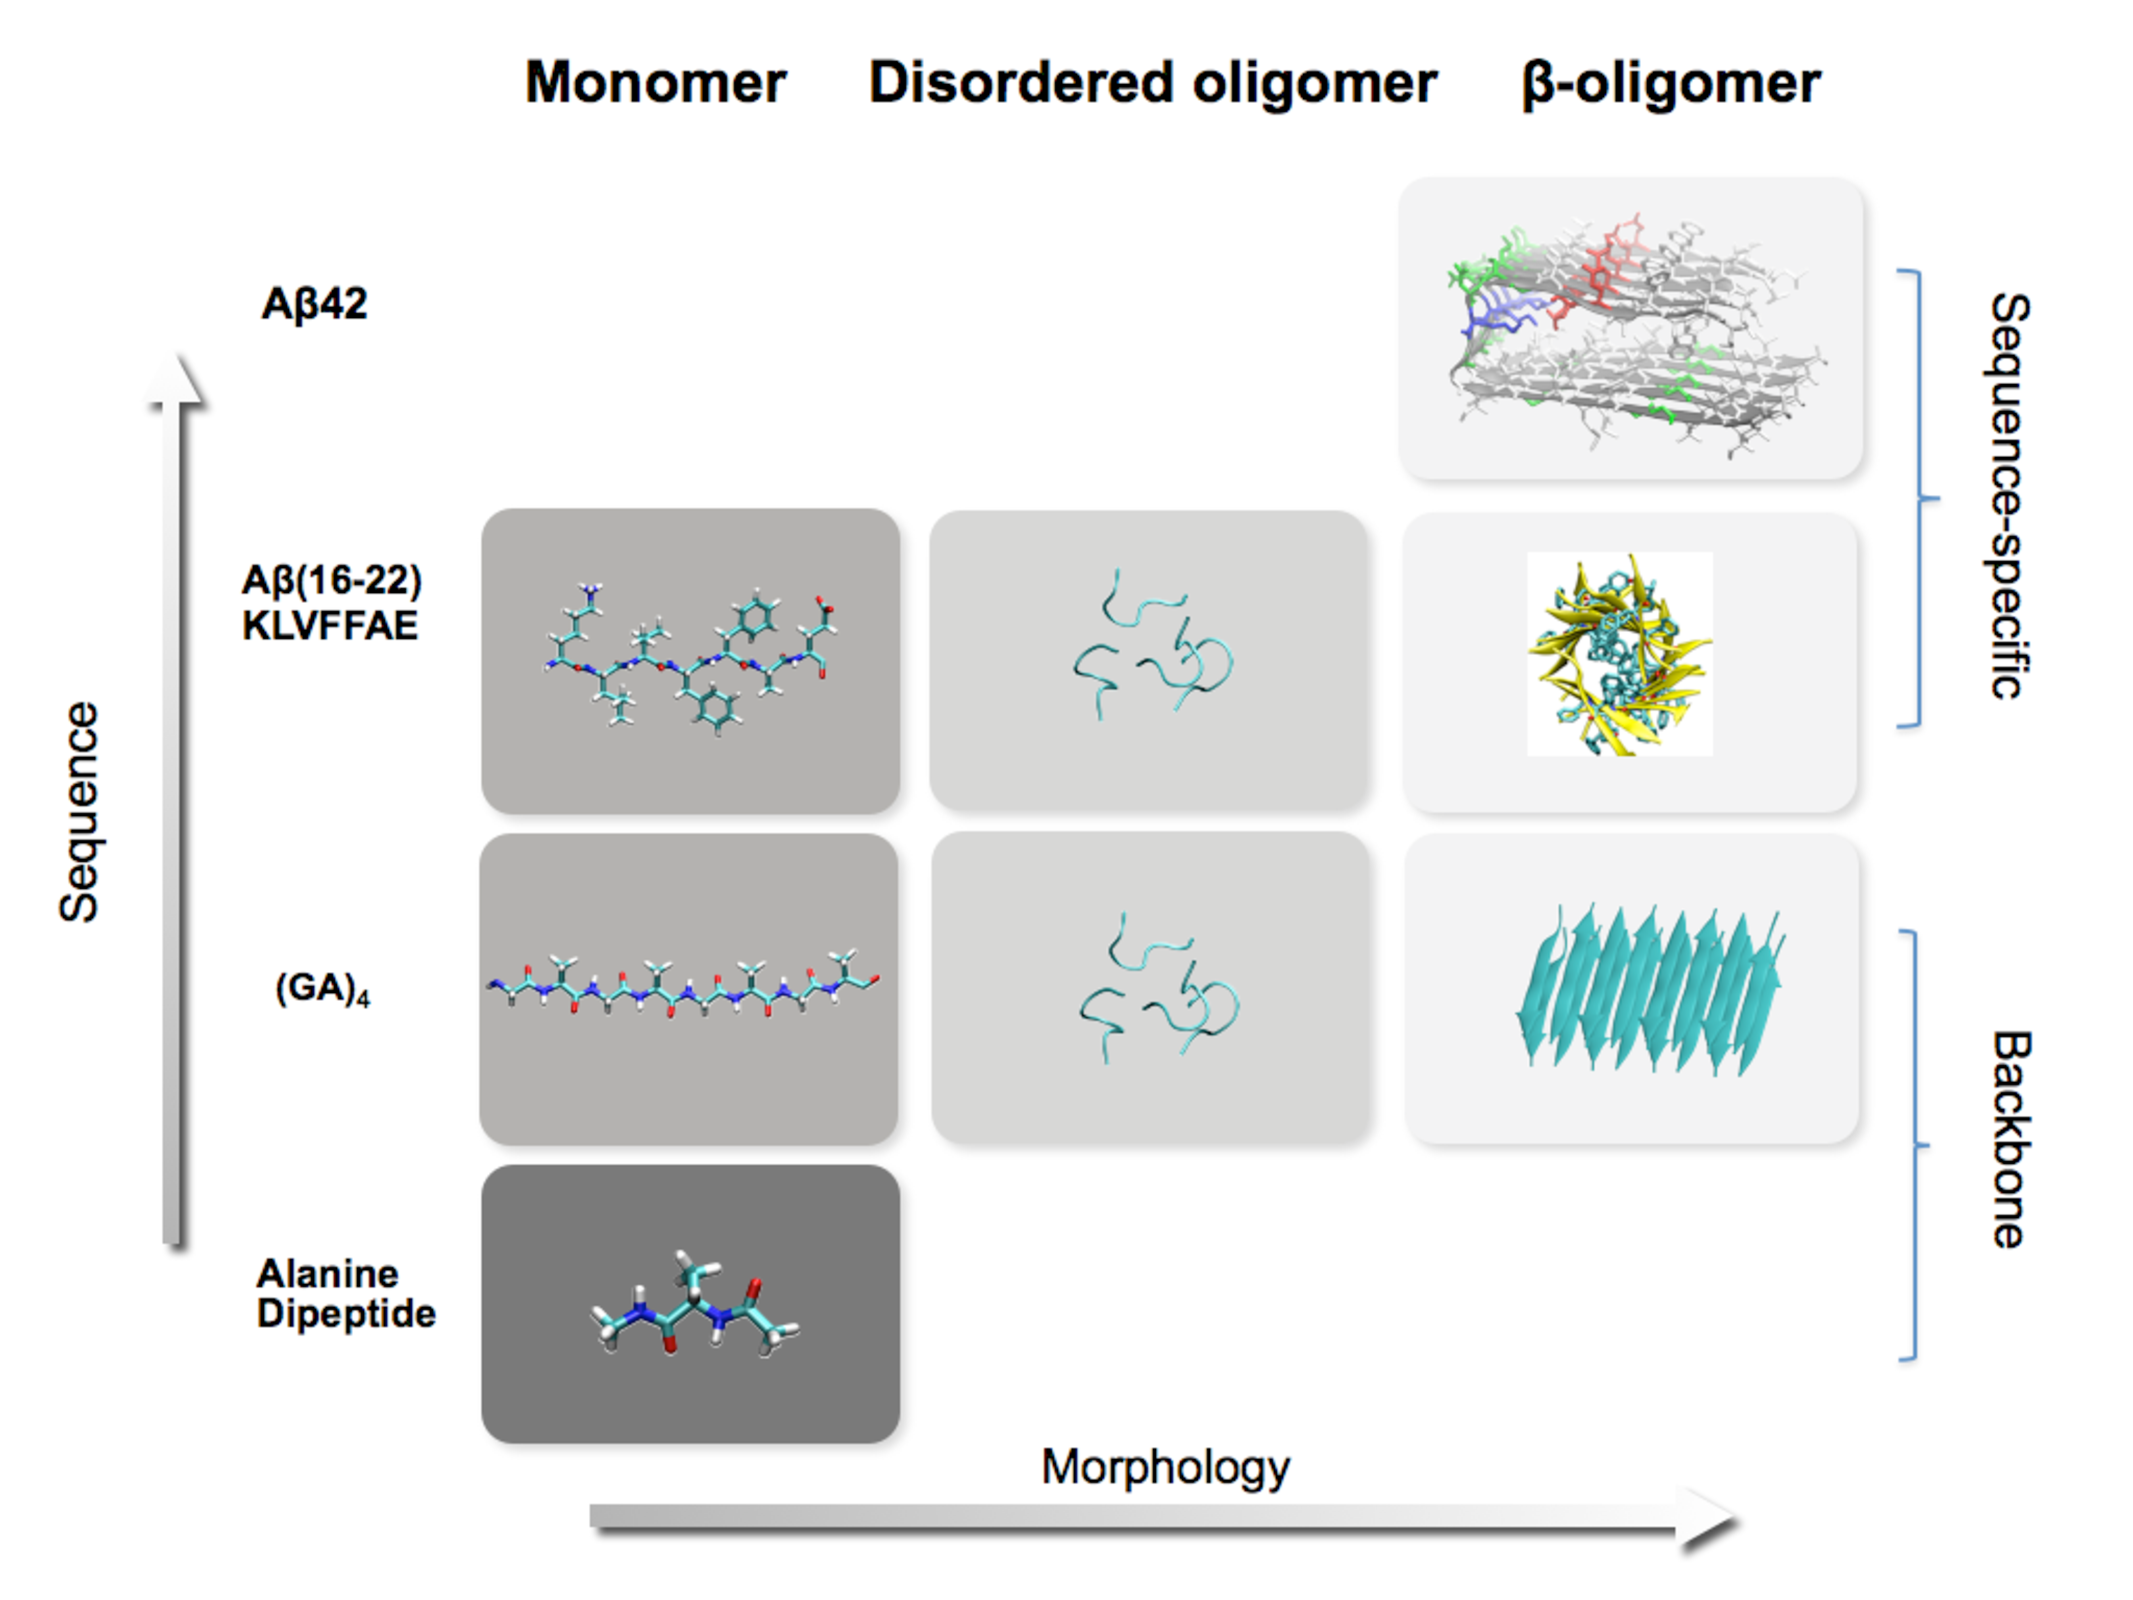
\includegraphics[width=6in]{figures/introduction/matrix.pdf}
\caption[Thesis study design and rationale]{A schematic of the different peptide sequences and aggregation states which form the basis of my studies involving inositol, arranged in order of sequence and structural complexity along the X and Y axes, respectively.}
\label{fig:rationale}
\end{figure}

% Amyloid fibrillation is a multi-stage process involving different species at each stage. Key states along the amyloid formation pathway involves the monomer peptide, small oligomeric aggregates, and ordered protofibrillar aggregates.  Hence in my study, I have chosen to study these systems in the presence of inositol.
% Determining the effect of inositol binding on the full-length A$\beta$ protein is computationally challenging and requires the use of many cores on high performance computing systems.
% In order to achieve the sampling necessary to obtain meaningful statistics from our simulations, we perform thousands of independent MD simulations of \textit{scyllo}- and \textit{chiro}-inositol with (1) single peptides; (2) small aggregates; and (3) large ordered aggregates of various amyloidogenic sequences (Figure~\ref{fig:rationale}). 
\subsection{Organization of thesis}
In Chapter 2, I review the details of molecular dynamics simulations, the central methodology throughout my dissertation. 
% Maybe this could be a perspectives paragraph describing what I did and how I discovered a more general use for what I've done.
% Each of the studies which constitutes my thesis follow a similar methodological approach. Systematic and comparative simulations.  Large number of repeated simulations using conventional sampling methods.  Low affinity interactions involving reversible binding.  The premise is that if a protein-ligand system has these characteristics, then one can conceivably apply the same methodology used for inositol to that system.

In Chapter 3, as a first step to investigate the stereochemistry-dependent effect on amyloidogenic peptide aggregation and morphology, I examined the effect of backbone interactions in polypeptide self-aggregation by systematically characterizing the binding equilibria of inositol with model peptides, alanine dipeptide (ADP), an amyloid-forming peptide (Gly-Ala)$_4$. 

In Chapter 4, I continue my investigation by characterizing the binding mechanism of inositol with peptide and aggregates of the amyloid-forming peptide fragment A$\beta$(16-22) (or KLVFFAE), a fibril-forming fragment thought to initiate amyloid formation in the full-length A$\beta$ peptide. Binding to grooves at the surface of $\beta$-sheet aggregates is found to play a central role in the activity of inositol. Taken together, the results presented in these chapters suggest that inositol is likely to act as a drug on protofibrillar-like aggregates. Accordingly, in Chapter 5, I characterize the binding mechanism of inositol with protofibrils of A$\beta$42.
% TODO: Need a better summary https://www.pivotaltracker.com/story/show/63666898
%\textit{I found that the binding modes of inositol with KLVFFAE adopt characteristic protein-carbohydrate binding modes.}

On the basis of my work involving inositol, a notable result is that the methodology utilized in these studies may be useful for investigating protein-carbohydrate binding mechanism in general. 
% Is there anything else?
In Chapter 6, applying the general methodology developed in this thesis, I characterize the binding modes and sites of monosaccharides glucosamine and GlcNac with  PgaB, a key protein responsible for the export of polysaccharides important for the formation of biofilms.  Using conventional sampling methods, I was able to map out a binding surface that predicted possible binding modes for the biologically-relevant polymer substrate of PgaB. The study presented in this chapter demonstrates that the methodology I have developed and utilized throughout this thesis can be successfully applied to characterize carbohydrate-binding proteins.  

%  Some where in here, maybe mention weak binding and how this relates to why I was able to use this methodology?

\begin{singlespace}
\addcontentsline{toc}{section}{Bibliography}
\bibliographystyle{elsart-num}
\bibliography{introduction}
\end{singlespace}


